% journal,10pt,draftclsnofoot,onecolumn
% \documentclass[journal,11pt,a4paper,onecolumn,draftcls]{IEEEtran}
\documentclass[a4paper]{IEEEtran}
\usepackage{graphicx, algorithm, algorithmicx, algpseudocode}
\usepackage{color}                    % For creating coloured text and background
\usepackage{amsmath,amssymb,amsfonts,epsfig} % Typical maths resource packages

\hyphenation{op-tical net-works semi-conduc-tor}
% TODO environment
\newcommand{\todo}[1]{\textsf{\emph{\textbf{\textcolor{blue}{#1}}}}}
\newcommand{\dean}[1]{\textsf{\emph{\textbf{\textcolor{green}{#1}}}}} 
\newcommand{\levin}[1]{\textsf{\emph{\textbf{\textcolor{red}{#1}}}}} 

\begin{document}

% can use linebreaks \\ within to get better formatting as desired
\title{The Circular Phase Transform for Estimation of Instantaneous Amplitude and Phase}

\author{Dean~R.~Freestone,~\IEEEmembership{Graduate Student Member,~IEEE,}
		David~B.~Grayden,~\IEEEmembership{Member,~IEEE,}
        Alan~Lai,~\IEEEmembership{Graduate Student Member,~IEEE,}
        Levin~Kuhlman,~\IEEEmembership{Member,~IEEE,}
        Timothy~S.~Nelson,~\IEEEmembership{Member,~IEEE,}
        Mark~J.~Cook,~\IEEEmembership{Member,~IEEE,}
        and Anthony~N.~Burkitt,~\IEEEmembership{Senior Member,~IEEE,}
        

\thanks{D.\ R.\ Freestone is with the Department
of Electrical and Electronic Engineering, University of Melbourne, VIC 3010, Australia, and The Bionic Ear Institute, 384-388 Albert Street, East Melbourne, VIC 3002, Australia {\tt\small dfreestone@bionicear.org}.}  % <-this % stops a space
\thanks{A.\ Lai is with The Bionic Ear Institute, 384-388 Albert Street, East Melbourne, VIC 3002, Australia}
\thanks{L.\ Kulhman is with the Department of Electrical and Electronic Engineering, University of Melbourne, VIC 3010, Australia}
\thanks{T.\ S.\ Nelson is with The Bionic Ear Institute, 384-388 Albert Street, East Melbourne, VIC 3002, Australia}
\thanks{M.\ J.\ Cook...}
\thanks{A.\ N.\ Burkitt is with the Department of Electrical and Electronic Engineering, University of Melbourne, VIC 3010, Australia, and The Bionic Ear Institute, 384-388 Albert Street, East Melbourne, VIC 3002, Australia}
\thanks{D.\ B.\ Grayden is with the Department of Electrical and Electronic Engineering, University of Melbourne, VIC 3010, Australia, and The Bionic Ear Institute, 384-388 Albert Street, East Melbourne, VIC 3002, Australia}

\thanks{Manuscript received Month Day, Year; revised Month Day, Year.}}


% The paper headers
\markboth{For submission to IEEE Transactions on Signal Processing}%
{Shell \MakeLowercase{\textit{et al.}}: Bare Demo of IEEEtran.cls for Journals}

\maketitle

\begin{abstract}
This paper introduces the Circular Phase Transform (CPT), a new technique for estimation of the instantaneous phase, frequency and amplitude from broadband, nonstationary oscillatory signals. The CPT performs an adaptive demodulation of the analytic signal in the phase-plane. Conceptually, the CPT is similar to the Hilbert-Huang transform (HHT), where the instantaneous phase is estimated from a signal that has been adaptively demodulated. However, unlike the HTT, the CPT does not require an iterative numerical demodulation, thus allowing for estimates of the instantaneous amplitude. In addition, the CPT provides a more local estimate of the instantaneous phase providing more accurate results. We show how the CPT can be used in an empirical mode decomposition and provide an example using an electroencephalography signal. 
\end{abstract}


% Note that keywords are not normally used for peerreview papers.
\begin{IEEEkeywords}
Time-frequency analysis, nonlinear signal processing, Hilbert-Huang transform.
\end{IEEEkeywords}

\IEEEpeerreviewmaketitle

\section{Introduction}
\IEEEPARstart{T}{he} concept of instantaneous frequency (IF) may seem an oxymoron. If frequency is defined as the number of repeating events per unit time, then it is difficult to conceptualize it as an instantaneous quantity. The definition of Fourier frequency for a stationary sinusoidal signal with multiple periods is clearly unambiguous. When considering a stationary sinusoid, IF can be thought of as an extension to Fourier frequency, where frequency is estimated using a small snap-shot (less than a full period) of the evolution of the phase (where the phase is defined as the entire argument of a cosine or sine function). The derivative of the instantaneous phase (IP) is the best estimate of the frequency at any local point in time. By defining the IF as the derivative of the IP, time-frequency properties of nonstationary, frequency modulated signals, such as chirps, can be estimated. For example, if one was interested in studying sea level fluctuations at a point within a swell, then the IF of the sea level measurements would describe the process. To demonstrate the procedure for calculating instantaneous amplitude, phase and frequency we first consider a narrow-band signal. The IP and IF can be estimated using the Hilbert transform, where the Hilbert transform of the signal $y(t)$ is defined as
\begin{equation}\label{eq:HilbertTransform}
\mathcal{H}y\left( t \right) = p.v.\int\limits_{ - \infty }^\infty  {y\left( \tau  \right)h\left( {t - \tau } \right)} d\tau,
\end{equation}
where $p.v.$ denotes the Cauchy principal value integral and $h\left( t \right) = {\left( {\pi t} \right)^{ - 1}}$. The analytic signal, $z(t)$, is defined as
\begin{eqnarray}\label{eq:AnalyticSignal}
z\left( t \right) &=& y\left( t \right) + j\mathcal{H}y\left( t \right) = r\left( t \right){e^{j\phi \left( t \right)}}\\
    &=& r\left( t \right)\left(\cos\left(\phi\left(t\right)\right) + j \mathcal{H}\cos\left(\phi\left(t\right)\right)\right),
\end{eqnarray}
where $r(t)$ and $\phi(t)$ are the instantaneous amplitude and phase, respectively, and $j=\sqrt{-1}$. The IF, $\omega(t)$, is defined as
\begin{equation}\label{eq:InstantaneousFreq}
\omega \left( t \right) = \frac{d\phi \left( t \right)}{dt} = \frac{d}{dt}\arctan\left(\frac{\mathcal{H}y\left( t \right)}{y\left(t\right)}\right).
\end{equation}
The IP and IF of a narrow-band signal can be uniquely defined if the conditions of the Bedrosian theorem~\cite{Bedrosian1963} are met, such that
\begin{equation}\label{eq:BedrosianCondition}
\begin{array}{*{20}{c}}
   {\mathcal{F}\left\{ {r\left( t \right)} \right\} = 0,} & {\,\left| \omega \right| > \omega_1,}  \\
   {\mathcal{F}\left\{ {\cos\left(\phi \left( t \right)\right)} \right\} = 0,} & {\left| \omega \right| < \omega_2,}  \\
\end{array}
\end{equation}
where $\mathcal{F}$ denotes the Fourier transform, $\omega$ denotes frequency where $\omega_2 \ge \omega_1 \ge 0$, and $\omega_1,\omega_2 \in \mathbb{R}{^ + }$. Eq.~\ref{eq:BedrosianCondition} states that the spectra of the IA and IP components of the signal must be disjoint, or not overlapping, for unique definition of the instantaneous properties. It can be interpreted as stating that the IA must be varying slower than the IP component. When these conditions are satisfied, the IP and IA components are separable, such that
\begin{eqnarray}\label{eq:SepAmpandPhase}
   \mathcal{H}y\left( t \right) &=& \mathcal{H}\left\{ {r\left( t \right)\cos \left( {\phi \left( t \right)} \right)} \right\} \nonumber \\
   &=& r\left( t \right)\mathcal{H}\left\{ {\cos \left( {\phi \left( t \right)} \right)} \right\}.
\end{eqnarray}
These conditions do not, however, guarantee that $r\left(t\right)\cos(\phi(t))$ and $r\left(t\right)\mathcal{H}\{\cos(\phi(t))\}$ form a quadrature pair when the instantaneous frequency or instantaneous amplitude is not constant~\cite{Nuttall1966}. This complicates the estimation of the instantaneous phase and will be discussed further in later sections. 

\begin{table*}[!ht]
\caption{
\bf{Notation}}
\begin{tabular}{|l|l|}
	\hline
	\textbf{Symbol} & \textbf{Quantity} \\ \hline
	$t$ & time \\ \hline
	$n$ & sample index \\ \hline
	$T_s$ & sampling period \\ \hline
	$F_s$ & sampling frequency \\ \hline	
	$f,\omega$ & Fourier frequency, Hertz and radians \\ \hline	
	$f_{max}$ & maximum Fourier frequency of interest in the signal \\ \hline
	$y(t),y(n)$ & test signal, continuous and discrete time \\ \hline
	$h(t)$ & Hilbert kernel ($1/\pi t$) \\ \hline
	$r(t), r(n)$ & instantaneous amplitude, continuous and discrete time \\ \hline
	$\phi(t),\phi(n)$ & instantaneous amplitude, continuous and discrete time \\ \hline
	$\mathcal{H}$ & Hilbert transform operator \\ \hline
	$\mathcal{F}$ & Fourier transform operator \\ \hline
	$\omega(t),\omega(n)$ & instantaneous frequency, continuous and discrete time \\ \hline
	$a$ & signal amplitude \\ \hline
	$x(t),x(n)$ & oscillatory component of signal, continuous and discrete time \\ \hline
	$x_0(t),x_0(n)$ & offset component of signal, continuous and discrete time \\ \hline
	$\varepsilon(t),\varepsilon(n)$ & signal noise or disturbance, continuous and discrete time \\ \hline
	$q$ & indexes of data segment used to fit circle, where $Q$ is total samples in the segment  \\ \hline
	$m$ & sets the size of the segment used to fit the circle ($m=m_{min},m_{min}+1,\hdots,m_{max}$) \\ \hline
	$\mathbf{p}_y(n)$ & point at sample $n$ in the phase-plane representation of the signal \\ \hline
	$\mathbf{p}_x(n)$ & point in the phase-plane representation of the oscillatory component of the signal \\ \hline 
	$\mathbf{p}_{x_0}(n)$ & point in the phase-plane representation of the offset of the oscillatory component of the signal \\ \hline  
	$\mathbf{a}(n)$ & normal vector to the tangent of the signal \\ \hline
	$\kappa$ & index for candidate circle fits \\ \hline
	$\zeta$ & circle center classifier \\ \hline
	$\beta$ & phase transition threshold \\ \hline 
	$\rho$ & oversampling parameter \\ \hline
	$\mathbf{v}_1(n,\kappa)$ & vector relating consecutive candidate circle parameters \\ \hline
	$\mathbf{v}_2(n,\kappa)$ & vector relating samples in the signal\\ \hline
	$d(n,\kappa)$ & relative distance mismatch \\ \hline
	$e(n,\kappa)$ & error in geometric distance to candidate circles \\ \hline
	$k,K$ & index and total number of intrinsic mode functions \\ \hline
	$s_{max,k}(n)$ & cubic spline interpolation through maxima of $y(n)$ (if $k=1$) or $x_{0,k}(n)$ (if $k>1$) \\ \hline
	$s_{min,k}(n)$ & cubic spline interpolation through minima of $y(n)$ (if $k=1$) or $x_{0,k}(n)$ (if $k>1$) \\ \hline
	$s_{ext,k}(n)$ & cubic spline interpolation used to find $r_k(n)$ in the CPT EMD \\ \hline
	$g(n,\kappa)$ & extrema of this guy are used for finding $s_{ext,k}(n)$ \\ \hline 
\end{tabular}
\begin{flushleft}This table provides a description of the notation used in this paper.
\end{flushleft}
\label{tab:Notation}
\end{table*}

Estimation of instantaneous properties from broadband signals is more complicated than the narrow-band case. Amplitude modulations and signal offsets in the time-domain lead to scenarios where the IF estimates are negative, according to the definition in Eq.~\ref{eq:InstantaneousFreq}. This is further illustrated in another paper regarding a different method for estimating phase and frequency~\cite{Huang1998}. Negative IF estimates arise when the analytic signal does not have an orbit enclosing the origin in the complex plane. Clearly, for the concept of IF to make sense it must be positive quantity. Therefore, from Eq.~\ref{eq:InstantaneousFreq}, it should be clear that the instantaneous phase of a signal should be monotonically increasing with time (except at $2\pi$ phase transitions if the phase is wrapped). To overcome this problem, a band-pass filter is typically used to extract narrow-band components before calculating the analytic signal in order to estimate the instantaneous properties. The filtering has an effect of re-centering the analytic signal in the phase-plane, ensuring the signal trajectory encloses the origin. Often this approach is undesirable since most naturally occurring signals do not have a stationary sinusoidal basis. 

%\section{Time-Frequency Distributions}
%This notion of instantaneous phase allows for the definition of a generalized (Cohen class) time-frequency distribution (TFD)~\cite{Cohen1995}. This provides an estimate of the energy in a particular frequency band at a particular time and is described as
%\begin{equation}\label{CohenClassTFD}
%\rho \left( {t,f} \right) = \int_{ - \infty }^\infty  {\int_{ - \infty }^\infty  {\int_{ - \infty }^\infty  {{e^{j2\pi v\left( {u - t} \right)}}g\left( {v,\tau } \right)} } } \,z\left( {u + {\raise0.7ex\hbox{$\tau $} \!\mathord{\left/
% {\vphantom {\tau  2}}\right.\kern-\nulldelimiterspace}
%\!\lower0.7ex\hbox{$2$}}} \right){z^*}\left( {u - {\raise0.7ex\hbox{$\tau $} \!\mathord{\left/
% {\vphantom {\tau  2}}\right.\kern-\nulldelimiterspace}
%\!\lower0.7ex\hbox{$2$}}} \right){e^{ - j2\pi f\tau }}dvdud\tau,
%\end{equation}
%where the kernel $g(v,\tau)$ dictates the type of TFD. The simplest case of this TFD is the Wigner-Ville distribution~\cite{Ville1958} (where $g(v,\tau) = 1$) and can be interpreted as the Fourier transform of the autocorrelation of the analytic signal. Importantly, the first moment of the time-frequency distribution corresponds to the Fourier frequency~\cite{Boashash1992}. TFDs of this class are very useful for IF estimates of frequency modulated (FM) signals, but do not provide estimates of the instantaneous phase and amplitude. Therefore, to fully describe instantaneous properties of signals we must use other methods.

% \section{Hilbert-Huang Transform}\label{HHTSection}
The Hilbert-Huang transform (HHT)~\cite{Huang1998} is a relatively new method for estimating IP and IA of nonlinear, nonstationary signals. Via a process known as empirical mode decomposition (EMD), the HHT decomposes a signal into the so-called intrinsic mode functions (IMFs). The trajectories of IMFs in the phase-plane have an orbit enclosing the origin, guaranteeing that the phase is monotonically increasing in time. Following this, the IP and IF can be defined using the Hilbert transform. The IMFs are extracted by an iterative process called `sifting', which can be considered as adaptive detrending or demodulating. The sifting algorithm involves finding a cubic spline interpolation through all local minima and another spline through local maxima, taking the average of the two splines (forming an adaptive trend), and subtracting this away from the original signal. The sifting typically requires several iterations, as the demodulation may introduce more extrema from inflections in the signal. The procedure continues until a stopping criterion is met, such that all modulations are removed from the signal (for example, the number of extrema equals the number of zero crossings, or is one less, and the splines are symmetric about the origin). Fig.~\ref{fig:HHTDemo} shows an example of the sifting process to extract the first IMF of a test signal
\begin{equation}\label{eq:FirstTestSig}
y\left( t \right) = a_1\cos \left(\omega_1t\right) + a_2\cos \left( \omega _2t \right),
\end{equation}
where $\omega = 2\pi f$, $f_1 = 7$ Hz, $f_2 = 17$ Hz, and $a_1 = f_1^{-1}$, $a_2=f_2^{-1}$. The example shows the four iterations, ordered from top to bottom, that were required to extract the first IMF. The sifting removes amplitude modulations and forms narrow-band components~\cite{Huang1998} allowing for estimation of the instantaneous properties using the Hilbert transform. The implementation of the HHT used in all of the examples in this paper is publicly available \dean{from the MathWorks File Exchange website~\cite{Tan2008}}. The HHT has proved very useful in a range of disciplines involving nonlinear, nonstationary signal processing. Applications include electroencephalography (EEG) signal analysis~\cite{Wang2008}, nonlinear system identification and structural health monitoring~\cite{Pai2008}. See~\cite{Huang2008,Huang2005a} for reviews.

A recent advance in the Hilbert-Huang transform involves normalization of the IMFs before computing the Hilbert transform~\cite{Huang2005}. The normalization is designed to separate the amplitude modulated and frequency modulated terms. By removing the IA component (or making it constant), the limitations stated in the Nuttall theorem~\cite{Nuttall1966} are addressed (improving the underestimates of the IF). However, the IF is still underestimated for non-trivial signals. This short-coming led to the development of the direct quadrature method, where the IP is estimated by simply taking the arccosine of the normalized IMFs. This provides a further improved IF estimate; however, problems occur with the estimation of the phase at times corresponding to the extrema of the signal if the normalization is $>1$, which is technically hard to achieve. This is because the arccosine of a signal is not defined (or complex) at points where the extrema are $>1$. 

A problem with the standard EMD is that it can not deal with noise or disturbances in a consistent manner, where noise and signal may get mixed into different IMFs~\cite{Wu2009}. The most recent development in the HHT is ensemble empirical mode decomposition (EEMD), which deals with this problem of intra-mode mixing~\cite{Wu2009}. The EEMD is inspired by the noise-added analyses of Flandrin et al.~\cite{Flandrin2005} and Glendhill~\cite{Gledhill2003} and extends findings from other recent studies concerning the statistical properties of the EMD and white noise~\cite{Flandrin2004,Wu2004}. The EEMD defines the a true IMF as the mean of an ensemble of realizations, each consisting of the signal with different additive white noise. By adding white noise to the data, the EEMD acts like a dyadic filter bank enabling the correct separation of scales.

\begin{figure}
\begin{center}
 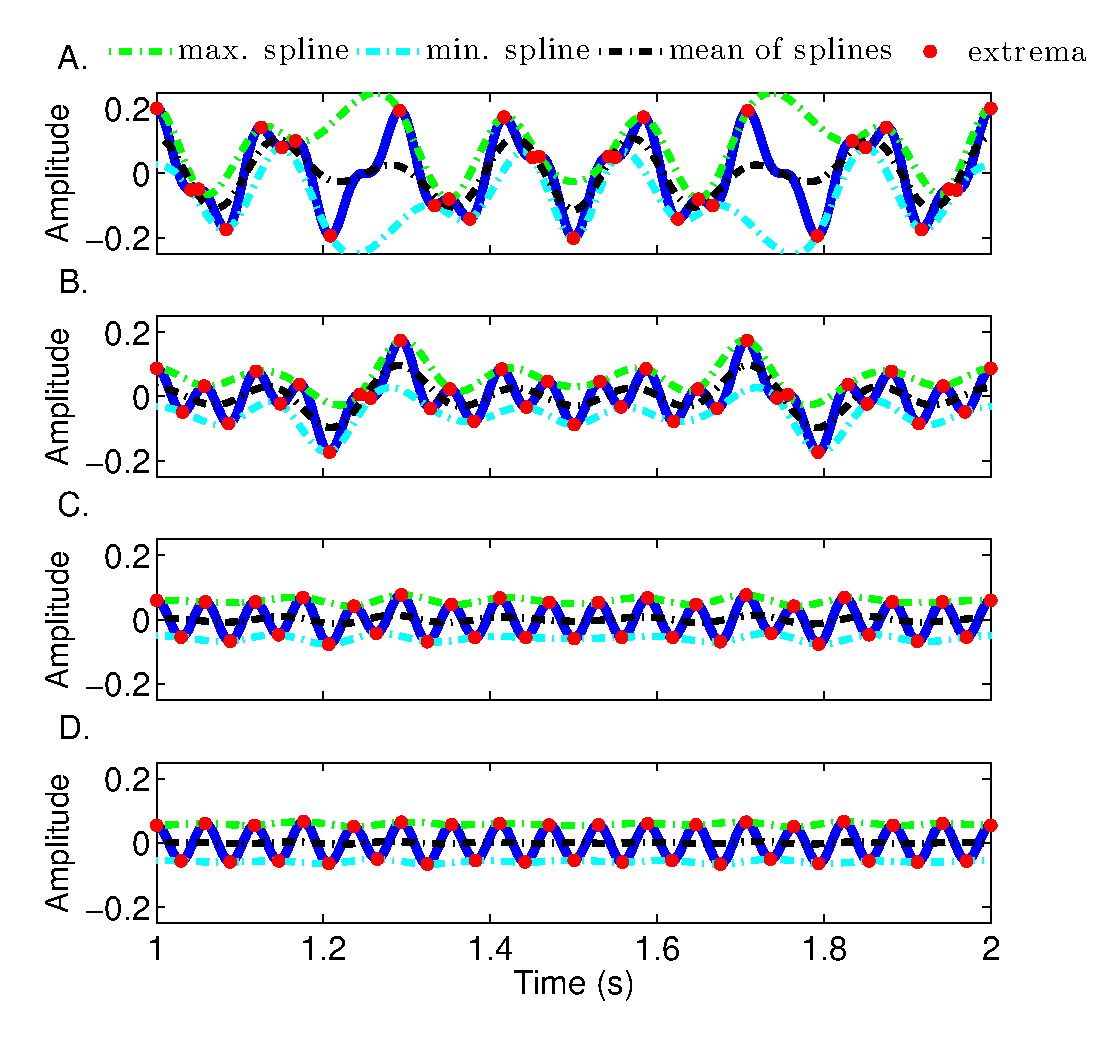
\includegraphics[scale=0.42]{./Figures/HHTDemo.eps}
 \caption[HHTDemo]{Illustration of extraction of the first IMF via the sifting process of the test signal from Eq.~\ref{eq:FirstTestSig}. Each plot is an iteration of the sifting algorithm, ordered from top to bottom. The results shown are from a signal of 3 seconds in duration. The first and last seconds are removed to alleviate problems with edge effects. Four iterations of the sifting process are required to find the first IMF. \textbf{A.} The original signal $y_1(t)$, the extrema points, and upper and lower splines. \textbf{B.} The signal $y_2(t)$ is the original signal detrended by the mean of the corresponding splines from \textbf{A.} \textbf{C.} the third iteration. \textbf{D.} the first IMF of HHT. Note how the amplitude information has been removed and the splines are symmetric about zero.}
\label{fig:HHTDemo}
\end{center}
\end{figure}

The HHT has proved very useful; however, there are several issues concerning the interpretation of IMFs. For example, the physical meaning of the IA estimates from the HHT is not clear. This is due to amplitude distortions caused by the iterative sifting process (the distortion of the IA can be seen in Fig.~\ref{fig:HHTDemo}). Furthermore, HHT IMFs are formed by interpolating extrema that may be relatively sparse in time, contradicting the notion of finding local instantaneous properties of a signal. These issues effect the standard HHT, the normalized HHT, and the direct quadrature methods since they all involve sifting. 
%Fig.~\ref{fig:HHTAmbiguity} provides an example of where inflection points cause problems for the HHT. For this example, we use the signal 
% \begin{eqnarray}\label{eq:HHTAmbiguityTestSig}
% y\left( t \right) &=& \cos \left( \psi \left( t \right) \right) \\
% \psi \left( t \right) &=& 2\pi ft + \cos \left( {2\pi ft} \right),
% \end{eqnarray}
% where $f=4$~Hz. The example illustrates how the sifting process can yield different results depending on where extrema occur. The inclusion of an extra maxima, by extending the data length by 100 ms (from Fig.~\ref{fig:HHTAmbiguity} B. to C.) changes the demodulation of the inflection points from phase distortions to full oscillations.
% 
% \begin{figure}
%     \centering
%     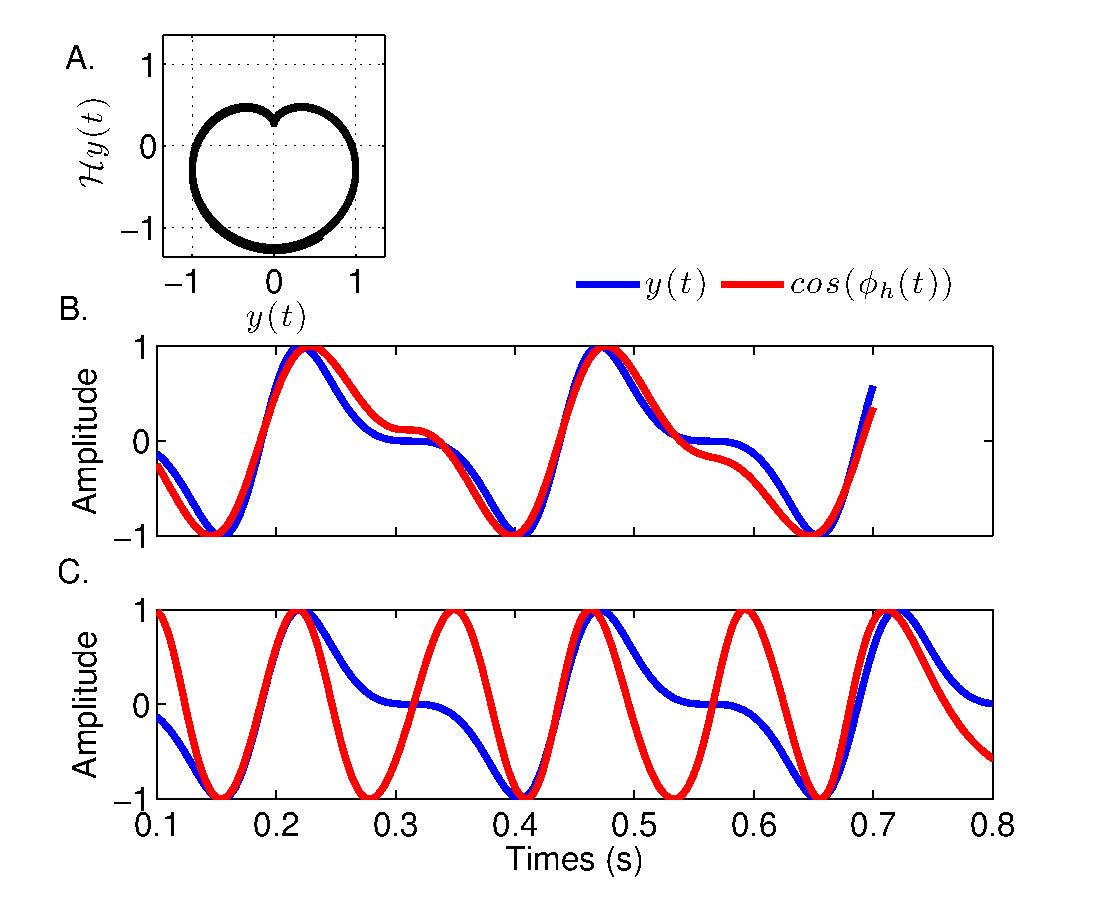
\includegraphics[scale=0.42]{./Figures/HHTAmbiguity}
%     \caption[HHTAmbiguity]{\textbf{A.} Phase plane representation of the test signal from Eq.~\ref{eq:HHTAmbiguityTestSig}. The upper zero crossing on the $\mathcal{H}y(t)$ axis shows a cusp that is generated by the inflection points in the signal. \textbf{B.} $y(t)$ plotted with the cosine of the instantaneous phase estimate of the first IMF computed with the HHT, $\phi_h(t)$. \textbf{C.} The same test signal and plot the same quantities as B., but $t$ is extended by 0.1~s. The estimate of the instantaneous phase is inconsistent between plots B. and C.}
%     \label{fig:HHTAmbiguity}
% \end{figure}

This paper extends the notion of instantaneous phase, frequency and amplitude for non-stationary signals through the introduction of the Circular Phase Transform (CPT). The CPT is conceptually related to the Hilbert-Huang Transform (HHT) in that it uses an adaptive demodulation technique to facilitate estimation of instantaneous signal properties. However, the CPT demodulates the signal in the phase-plane by finding local circle fits, allowing for more accurate phase and amplitude estimates. The paper is laid out as follows. Section~\ref{sect:CPTDescriptionSection} explains the concepts and theory underpinning the CPT. Section~\ref{sect:ComputingCPTSection} describes the procedure for computing the CPT. Section~\ref{sect:NoisySignalsSection} demonstrates how the CPT performs with noisy signals and illustrates how to select appropriate parameters for computing the transform. Section~\ref{sect:CPTEMDSection} shows how the CPT can be used to create an EMD that does not rely on the sifting process. %Section~\ref{sect:PhasePlaneCuspsSection} shows how inflections in a time series, or equivalently, phase-plane cusps pose major challenges for estimating IP. Section~\ref{EEGExampleSection} provides a practical example of the CPT EMD using an EEG signal. 
The Discussion and Conclusion follow in Sections~\ref{sect:DiscussionSection} and~\ref{sect:ConclusionSection}, respectively. 

\section{The Circular Phase Transform}\label{sect:CPTDescriptionSection}
The Circular Phase Transform (CPT) is a new method for estimating the instantaneous phase and amplitude (IP and IA) from nonstationary signals. Using the derivative of the IP the instantaneous frequency (IF) can be calculated. The CPT is an alternative to the HHT that provides improved estimates of instantaneous properties of signals by obtaining more local IA and IP estimates. The CPT models a signal's local trajectory in the phase-plane as an arc of a circle. The circle center provides a new reference point for calculating the IP and IA, thereby acting as an adaptive demodulation.

For smooth and continuous oscillatory signals, the local (infinitesimally small) phase-plane trajectory can be accurately described by the arc of a circle. For this class of signal, we can think of the IF as the reciprocal of the time taken to complete the circular orbit at its current rate of change and trajectory (following the arc) in the phase-plane. In other words, it is the best estimate of the instantaneous frequency, since a sinusoid is a circle in the phase-plane. Fourier analysis measures the correlation of the signal in the phase-plane to trajectories of unit circles with a harmonically-related set of frequencies. The CPT estimates circle parameters (radius and center), allowing them to vary at each time sample, thus establishing a basis that is adaptive. In this way, a general platform to establish the notion of IF is provided.

With sufficient sampling and signal-to-noise ratio, the instantaneous properties described by an arc may be estimated from a discrete time series using circle fitting methods. The uniqueness of the phase-plane representation of a signal is guaranteed if the conditions of the Bedrosian theorem~\cite{Bedrosian1963} are met, and the uniqueness of the IA and IP estimates are inherent in circle fitting methods. In addition, the locally circular representation of the phase-plane trajectory enforces a quadrature structure on the analytic representation of the signal.

The CPT requires the signal to satisfy three conditions in addition to the condition stated by the Bedrosian theorem (Eqs.~\ref{eq:BedrosianCondition}). The signal must be 1) smooth and continuous, 2) oscillatory, and 3) mono-component. The third condition allows for physical interpretation of the CPT. A common way to define a signal as being mono-component is to use a particular basis and time scale as a reference~\cite{Boashash1992,Cohen1995}. This definition is not appropriate here, since we are dealing with instantaneous quantities, where time scales are continuously changing and the basis is arbitrary. Therefore, we define a signal as being mono-component if it can be sufficiently described by a scalar quantity when it is sampled from a vector field. For example, when considering sea level measurement, the signal is mono-component if the surface of the sea beneath the measurement sensor is uniform in height (or can be approximated by an average). This condition does not restrict the generator of a signal to a single source. Sea level will be affected by waves from all directions but, if the measurement is descriptive of the process at a single point in space, we can consider it mono-component. Together, the conditions ensure the signal has an oscillatory component that has a phase that is monotonically increasing in time (except at $2\pi$ transitions) and a trajectory in the phase-plane that encloses the origin. 

Under our standing assumptions, the signal in the phase-plane can be modeled as
\begin{align}\label{eq:SignalModel}
y\left( t \right) &= x\left( t \right) + x_0\left( t \right) + \varepsilon \left( t \right) \\
\mathcal{H}y\left( t \right) &= \mathcal{H}(x\left( t \right) + x_0\left( t \right) + \varepsilon \left( t \right)),
\end{align}
where $x(t) \in \mathbb{R}^1$ is an oscillatory component, $x_0(t) \in \mathbb{R}^1$ denotes an offset (or adaptive trend) and $\varepsilon(t) \sim \mathcal{N}(0,\sigma^2)$ represents process or measurement noise. The oscillatory component, $x(t)$, can be thought of as being analogous to the first IMF of the HHT and can be parameterized by IA and IP as
\begin{equation}\label{eq:InstAmplitudeAndPhase}
    x\left( t \right) = r\left( t \right)\cos \left( {\phi \left( t \right)} \right),
\end{equation}
where $r(t)$ denotes the IA and $\phi(t)$ denotes the IP. 

In the noise-free case 
\begin{align}
	x\left( t \right) &= y\left( t \right) - x_0\left( t \right) \\
	\mathcal{H}x\left( t \right) &= \mathcal{H}\left(y\left( t \right) - x_0\left( t \right)\right)
\end{align}
and the IA is
\begin{equation}\label{eq:IADef}
    r\left( t \right) = \left( x^2(t) + \mathcal{H}x^2(t)\right)^{1/2}.
\end{equation}
For a smooth continuous oscillatory signal, the IA will satisfy
\begin{equation}\label{eq:IAlimitingCase}
\mathop {\lim }\limits_{\tau  \to 0} \left( r\left( t \right) - r\left( t + \tau \right) \right) = 0.
\end{equation}
Naturally, it follows that for a small finite time interval, $\Delta t$, we have
\begin{equation}\label{eq:IA_small_time_interval}
    r(t)-r(t-\Delta t) < \eta,
\end{equation}
where $\eta \in \mathbb{R}$ is a small constant. Equations~\ref{eq:IADef}, \ref{eq:IAlimitingCase}, and \ref{eq:IA_small_time_interval} simply state that given a sufficiently small segment of data the local oscillatory component, $x(t)$, can be approximated by an arc of a circle in the phase-plane or, equivalently, a sinusoid in the time domain. In the noise-free case, the IP of $x(t)$ is
\begin{equation}\label{IPdef}
    \phi \left( t \right) = \arctan \left( \frac{\mathcal{H}x\left( t \right)}
    {x\left( t \right)} \right).
\end{equation}
% this bit is commented out because we are not comparing the CPT to the DQ method
% ~~~~~~~~~~~~~~~
% An example of an IF estimate using the CPT is provided in Fig.~\ref{CompareWithDQ}, where we compare the Hilbert-Huang transform, the direct quadrature method (DQ), and the CPT. For this example, we used the test signal 
% \begin{equation}\label{DQTestSignal}
% y(t) = e^{-t/256}sin\left(\frac{\pi t}{32} + 0.3sin\left(\frac{\pi t}{32}\right)\right).  
% \end{equation}
% This test signal was chosen since it was used as an example in~\cite{Huang2008} for demonstrating problems of having non-quadrature Hilbert transforms, which results in an underestimate of the IF when using the HHT. The DQ method and the CPT both provide very good IF estimates. The HHT IF estimates are inaccurate due to having a non-quadrature analytic signal for the IMF. The DQ method overcomes the limitations described in the Nuttall theorem via normalizing the IMFs prior to computing the analytic signal. The CPT overcomes the limitations of the Nuttall theorem by enforcing a circular structure in the phase-plane. The DQ method has some minor problems in estimating the IF at points corresponding to extrema of the time-series. This is a consequence of the normalization procedure. 
% ~~~~~~~~~~~~~~~
Modelling the signal trajectory as an arc of a circle in the phase-plane enables the inclusion of a disturbance term, allowing for noise to be dealt with in a consistent manner. Further more Rau Cramer lower bound... In addition, the CPT does not rely on sifting, meaningful IA estimates are obtained.
% advantage of the CPT method over the HHT is that it does not rely on the sifting process, allowing for inflections to be handled in a more consistent manner. Another 

% this bit is commented out because we are not comparing the CPT to the DQ method
% ~~~~~~~~~~~~~~~
% \begin{figure*}
%   \centering
%   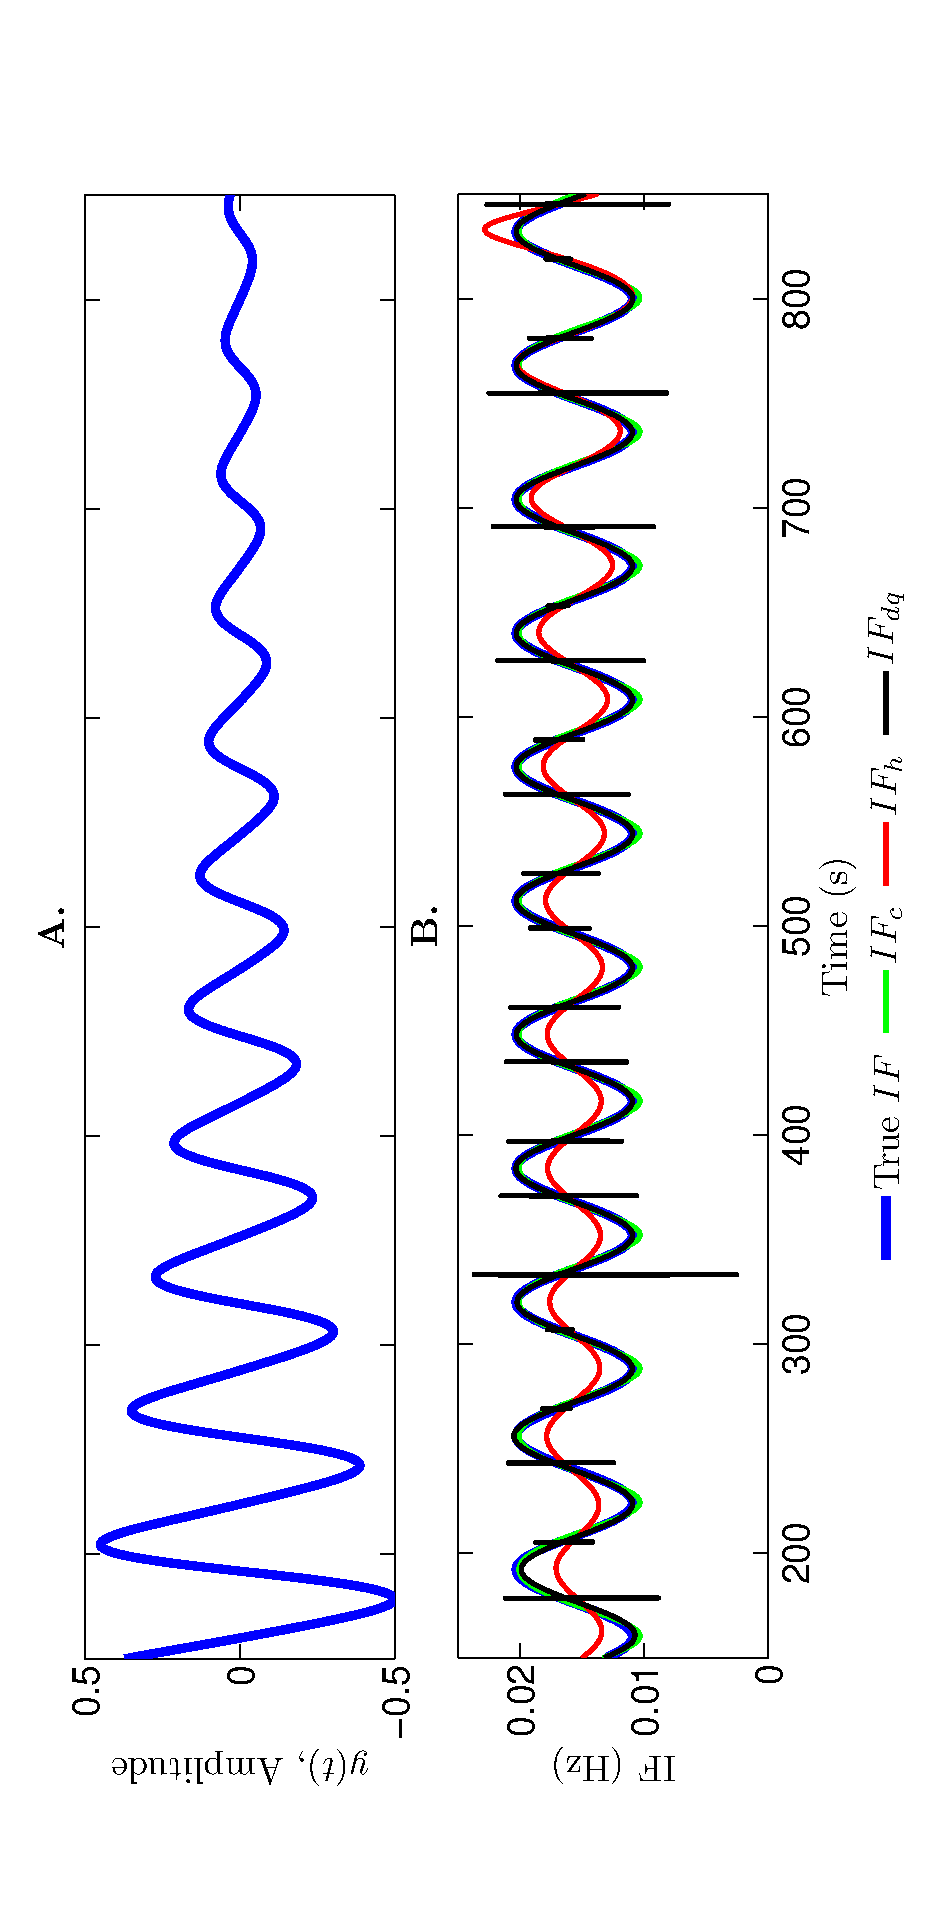
\includegraphics[scale=0.4,angle=-90]{IF_comparison_with_dq}
%   \caption[CompareWithDQ]{\textbf{A.} The test signal described by Eq.~\ref{DQTestSignal}. \textbf{B.} \todo{Remove legend and describe the colors. Add zoomed subplot on RHS. Point out how things are overlapped. Try different line widths for true IF. Discuss glitches with DQ in text and cite the paper.} Illustration of the IF estimates for the CPT, HHT, and DQ methods, compared to the true IF.}
%   \label{CompareWithDQ}
% \end{figure*}
% ~~~~~~~~~~~~~~~

\section{Computing the CPT}\label{sect:ComputingCPTSection}

The Circular Phase Transform is principally a circle fitting procedure. The steps of the CPT algorithm are presented in Algorithm~\ref{CPTAlgorithm}. After preprocessing and computing the Hilbert transform of the signal, to get a phase-plane representation, the algorithm consists of three steps for each sample in the time series. 
The first step, described in Section~\ref{sect:FindingArc}, is to find a set of points around the current sample to specify an arc of a set length. The second step is to implement a standard circle fitting technique to the arc, for each point in the time series. The circle fitting algorithm provides an estimate of $r(t)$ and $x_0(t)$ for each sample. The circle parameters can then be used to estimate $\phi(t)$. The third step, described in Section~\ref{sect:DetectingInvalidParameters}, checks the validity of the circle fits using prior knowledge of the data structure. After unwrapping the valid IP estimates, the invalid parameters are rejected and recovered via interpolation. 

\subsection{Determining the Arcs for the Circle Fits}\label{sect:FindingArc}
The number of points in a specified arc length of $\psi$ about a point of interest depends on the sampling rate and the frequency content of the data. It is assumed to be unknown and to vary throughout the time series. Therefore, the points that describe the prescribed arc must be found empirically.

To show how the arc is formed, we will first consider a noise-free sinusoid of unknown frequency. The point of interest in the phase-plane representation of the signal can be described in vector form as
\begin{equation}
	\mathbf{p}_y(n) = \left[y\left(n\right),\mathcal{H}y\left(n\right)\right]^{\top}.
\end{equation}
The arc used to fit the circle for this point is described by the set of consecutive neighbouring points
\begin{equation}
	\mathbf{P}_y(n) = \left[\mathbf{p}_y(n-b),\hdots,\mathbf{p}_y(n),\hdots,\mathbf{p}_y(n+f)\right],
\end{equation}
where $b$ and $f$ are integers that specify the edges of the arc for the point at $n$. Now we define the vectors that describe the points at the edges of the arc relative to the point of interest as
\begin{align}
	\mathbf{p}_b(n) &= \mathbf{p}_y(n-b)-\mathbf{p}_y(n) \\
	\mathbf{p}_f(n) &= \mathbf{p}_y(n+f)-\mathbf{p}_y(n).
\end{align}
The arc length is measured using the angle between these two vectors by
\begin{equation}
	\theta = \arccos\left(\frac{\langle\mathbf{p}_b(n),\mathbf{p}_f(n)\rangle}{\|\mathbf{p}_b(n)\| \|\mathbf{p}_f(n)\|}\right),
\end{equation}
where given for a given $b$ and $f$, the measured arc length, $\hat\psi$, is calculated by
\begin{equation}\label{eq:theta_2_psi}
	\hat\psi = 2(\pi-\theta).
\end{equation}
Note, $\psi$ must be $<2\pi$ for $\theta$ to be unique. The desired arc length is found (for each point) by systematically incrementing $b$ and $f$ until $\hat\psi > \psi$. If $\hat\psi < \psi$ the integers that define the boundary of the arc, $b$ and $f$, are incremented with the goal that
\begin{equation}\label{eq:balanced_distances}
	\|\mathbf{p}_f(n)\| = \|\mathbf{p}_b(n)\|.
\end{equation}
If $\|\mathbf{p}_f(n)\| < \|\mathbf{p}_b(n)\|$, then $f$ is incremented, otherwise $b$ is incremented. Following this, the arc is approximately symmetric about the point $\mathbf{p}_y(n)$. 

Now consider a noisy sinusoid. In this case the measured arc length, $\hat\psi$, may sporadically increase above the desired arc length, $\psi$, due to fluctuations from the disturbance. Therefore, in our implementation we require $\hat\psi$ to be greater than $\psi$ for multiple consecutive samples. This number of samples is a free parameter that depends on the sampling rate and the SNR of the time series. 

Now consider a more complex time series with inflections. In this case the problem of finding a specified arc length becomes more complicated as inflections in a time series are cusps in the phase-plane representation. At the point of a cusp, the phase-plane trajectory does not follow an arc of a circle. Therefore, the arc used to fit the circle should not be spanning a cusp and the desired arc length, $\psi$, will not be achievable. Nevertheless, a shorter arc length not spanning the cusp may still provide a good circle fit. For this scenario, $\theta$ is not necessarily monotonically decreasing as $b$ or $f$ is incremented. In the noise-free case, cusps can be detected by checking for increases in $\theta$ as $b$ or $f$ is incremented. However, if there is a high level noise is present, cusps become hard to discern. For low-noise signals cusps can be detected if $\theta$ grows whilst $b$ or $f$ are incremented. The cusp detection threshold will be signal dependant, thus is a  parameter to be set by the user. If a cusp is detected, then the arc will be chosen such that it does not cross the cusp.
 

 


% The algorithm fits circles to segments of data (using a sliding window) allowing for different  arc lengths at each sample, by fitting circles to a range of candidate segment lengths and selecting the best one. The concavity of the arc is checked for by ensuring that the fitted circle center is on the correct side or the arc; this is done by estimating the tangent, and thereby the normal, vector. In addition, the IP corresponding to the the candidate circles is checked, making sure the IP is monotonically increasing in time. The best circle fit (according to our criteria) is selected from the valid candidates (with varying arc lengths) and the corresponding parameters are used to describe the instantaneous properties of the signal. Finally, missing data points that did not satisfy the criteria inserted by interpolation.

\subsection{Circle Fitting Procedure}\label{sect:CircleFittingProcedure}
% From this point on, the signal, $y(t)$, will be referred to as a discrete time series $y(n)$, where $n$ indexes the samples and $T_s$ is the sampling period. The data segments used to find the candidate circle fits for sample $n$ are described by the set of points
% \begin{equation}\label{eq:DataSegment}
% \{\left(y\left(q\right),\mathcal{H}y\left(q\right)\right)  \,\forall q \ | \, q \in [n-m_b,n+m_f]\},
% \end{equation}
% where $m\in\mathbb{N}^+$ and $m=m_{min},..,m_{max}$ sets the segment lengths, which are $2m+1$ samples. The minimum size of a segment to fit a circle from data that is not a perfect circle is 4, therefore $m_{min}>1$. The segments are described as being symmetric about the sample of interest, $n$, for clarity of explanation. This is not a requirement for the transform where, for example, an asymmetric or randomly drawn set of samples about the sample of interest may be used to find the candidate circles. By using a range of candidate circle fits, nonstationarity can be accounted for. For example, if a section of a time series has a slowly varying IP and IA, then a larger arc, or more samples, should be used to fit a circle (if there is noise present) than if the IP and IA were varying faster.

Many linear and nonlinear least-squares techniques exist for fitting circles to noise-corrupted data. These methods provide estimates of the circle radius and center. Linear methods have closed-form solutions and nonlinear methods are calculated numerically (see~\cite{Chernov2005} for a review). The circle fitting method that we have applied in this paper is the Taubin method~\cite{Taubin1991}. This method was chosen due to the good performance when using noisy data with small arc lengths and its wide acceptance in the circle fitting literature.

By estimating a circle that best fits the data segment in a least squares sense, the discrete IA and IP can be calculated. Provided the circle estimate is accurate, the IP is monotonically increasing in time and the oscillatory component has a phase-plane trajectory that encloses the origin. This allows the IP to be unwrapped unambiguously, where any decrease in the wrapped phase is a $2\pi$ phase transition. An example of the a circle fit is shown in Fig.~\ref{fig:MappingDemo}.

\begin{figure}
    \centering
    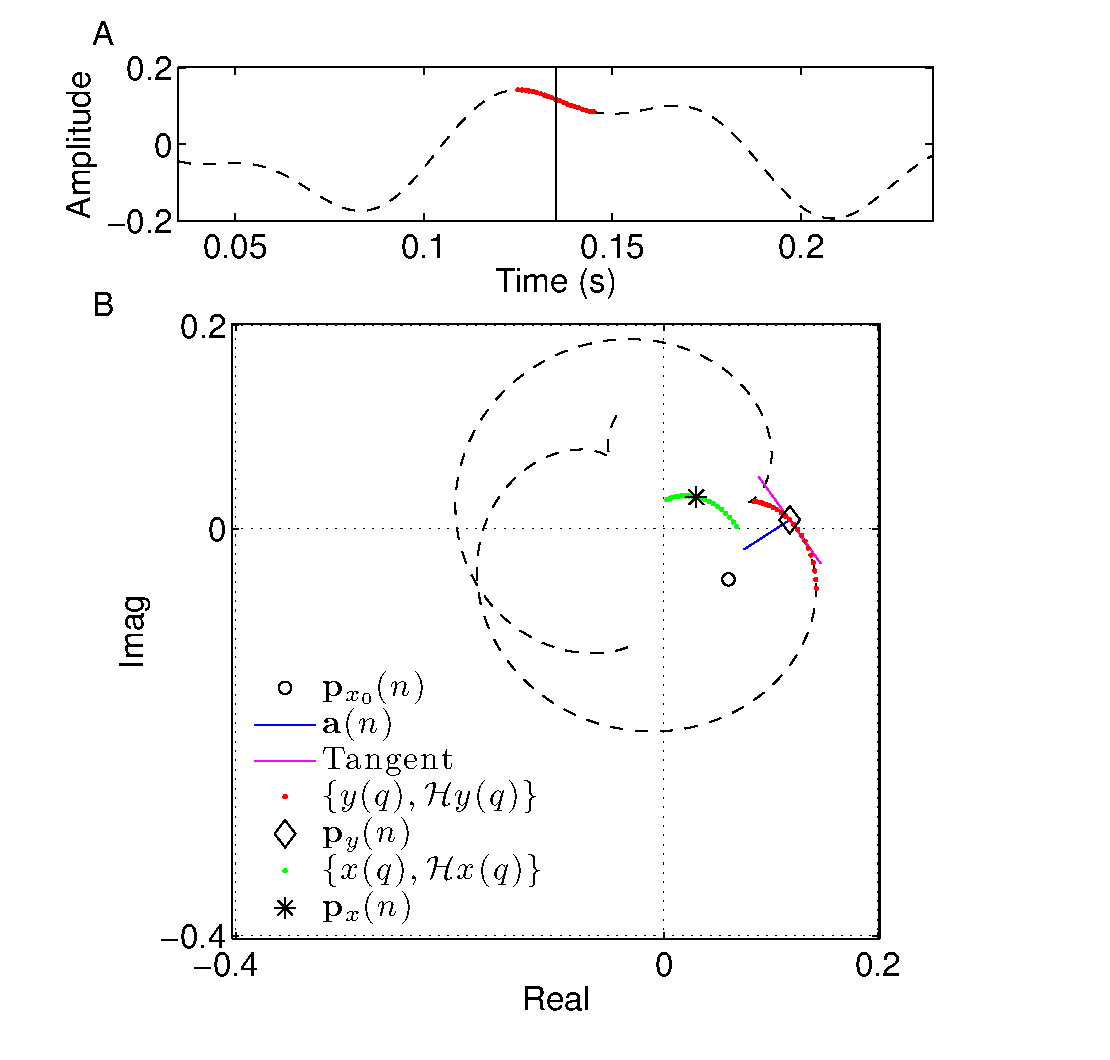
\includegraphics[scale=0.42]{./Figures/MappingDemonstration.eps}
    \caption[MappingDemo]{Demonstration of the Circular Phase Transform. \textbf{A.} A discrete time series $y(n)$ used to compute the transform. The black vertical line highlights the current sample, or point of interest and the red points in the time series highlight the segment used to compute the CPT. \textbf{B.} The phase-plane representation of the signal $y(n)$ (in blue) and the transformed phase-plane representation (in green). Note how the cycloid of the original signal was mapped to enclose the origin. The red data points highlight the segment of data used to fit the circle. The open circle shows the current sample, or point of interest. The red cross shows the center of the fitted circle for the current mapping. The Fig. also show an estimated tangent and normal vector used to detect incorrect mappings. The distance between the black and blue stars reflect the relative distance mismatch (normalized).}
    \label{fig:MappingDemo}
\end{figure}

\subsection{Detecting Invalid Parameters}\label{sect:DetectingInvalidParameters}
To accurately approximate the phase-plane trajectory of a nonstationary signal by an arc of a circle it is desirable to use small segments of data. However, when using fewer points and smaller arc lengths, noise has a larger effect on the result. Therefore, a series of checks is used to prevent errors. 
\subsubsection{Incorrect Circle Center Identification}
Any bounded oscillatory signal will have a closed trajectory in the phase-plane. Therefore, the fitted circle centers (signal offsets) should be confined to one side of the arc. However, errors can occur when fitting circles to noisy data. Noise may make a concave arc appear to be convex (or vice-versa), resulting in the circle center being mapped to the incorrect side of the arc. A method to prevent circle centers being mapped to the incorrect side is to use the local tangent of the signal as a separating line. If candidate circle centers are on the incorrect side of the tangent, they are rejected. This can be detected by computing the inner product of the normal vector to the tangent and the circle center estimate. 

The direction of the tangent of the phase-plane trajectory of the signal is approximated by 
\begin{equation}
	\mathbf{g}(n) = \mathbf{p}_y(n + f_t) - \mathbf{p}_y(n - b_t),
\end{equation}
where $f_t$ and $b_t$ is the number of samples forward and backward, respectively, from the point of interest to estimate the tangent. For noisy signals, the points used to estimate the direction of the tangent should be at the edges of an arc length of $\pi$ around the point of interest. This minimizes the effect of noise. The points $n+f_t$ and $n+b_t$ are found in the same manner as finding the arc length for the circle fit, described in Sect.~\ref{sect:FindingArc}. To classify incorrect centers, the normal vector to the tangent is found using a 90 degree rotation of $\mathbf{z}(n)$ by
\begin{equation}
	\mathbf{a}\left(n\right) = \left[\begin{array}{cc}
	0 & -1 \\
	1 & 0\end{array}\right]\mathbf{g}(n).
\end{equation}
The estimated oscillatory component, $\hat{x}(n)$, and the associated circle center (or offset), $\hat{x}_0(n)$, can be written in vector form as
\begin{align}
	\mathbf{p}_x(n) &= \left[\hat{x}\left(n\right),\mathcal{H}\hat{x}\left(n\right)\right]^{\top} \\ 
	\mathbf{p}_{x_0}\left(n\right) &= \left[\hat{x}_0\left(n\right), \mathcal{H}\hat{x}_0\left(n\right)\right]^{\top}. 
\end{align}
Invalid candidate circle centers are detected using 
\begin{equation}
    \zeta(n) = \mathbf{a}\left( n\right)^{\top}\left( \mathbf{p}_{x_0}\left( n \right) - \mathbf{p}_x\left( n\right) \right),
\end{equation}
where an incorrect estimate is detected with the condition
\begin{equation}\label{eq:IncorrectSideClassifier}
    \zeta(n) < 0.
\end{equation} 

If estimated circle center does not satisfy this condition at a particular point, then the IP and IA cannot be estimated for that sample using this method. These values must be interpolated at the completion of the estimation procedure for all samples in the time series. 

\subsubsection{Incorrect Phase Progression}
The candidate circle fits are further constrained using prior information of the phase progression. From our fundamental definition of IP, the unwrapped phase is monotonically increasing in time except at $2\pi$ phase transitions. A phase increment threshold and a phase transition threshold can be derived given knowledge of the sampling rate and the maximum frequency of interest in the signal. To begin the derivation, an oversampling parameter is defined based on the Nyquist sampling theorem as
\begin{equation}
	\rho\triangleq\frac{F_s}{2f_{max}},
\end{equation}
where $\rho \in \mathbb{R} \ge 1$, $F_s$ is the sampling frequency, and $f_{max}$ is the maximum frequency of interest in the signal. Under the assumption that the IP estimate at sample $n-1$ is accurate, the phase estimate at sample $n$ should satisfy
\begin{equation}
	0 < \hat\phi(n)-\hat\phi(n-1) < \beta
\end{equation}
where 
\begin{equation}
	\beta = \frac{\pi}{\rho}
\end{equation}
Now consider the next IP estimate at the sample $n+1$. The error in the previous estimate is bounded by $\beta$, so the error in the next estimate must satisfy
\begin{equation}\label{eq:Prior1}
	0 < \hat\phi(n+1)-\hat\phi(n) < 2\beta
\end{equation} 

At a $2\pi$ phase transition, the maximum phase decrement in radians is
\begin{equation}
	\alpha=2\beta-2\pi.
\end{equation}
Following this, the phase evolution should also satisfy
\begin{equation}\label{eq:Prior2}
\hat{\phi} \left( n \right) - \hat{\phi} \left( n-1\right) \le \alpha. 
\end{equation}

If the conditions from Eqs.~\ref{eq:IncorrectSideClassifier},~\ref{eq:Prior1}, and~\ref{eq:Prior2} are not satisfied from the previous sample, $n-1$, than parameters corresponding to an earlier sample, $n-p$, where the conditions are satisfied is used. Following this, we need to re-evaluate the thresholds used in Eq.~\ref{eq:Prior1} and~\ref{eq:Prior2} to
\begin{align}
	\beta_p &= \frac{p\pi}{\rho} \\
	\alpha_p &=2\beta_p-2\pi.
\end{align}
Note that in order for the threshold $\alpha_p$ to be useful, it must be negative. Therefore, there is a limit on the size of $p$ where $\alpha_p$ is meaningful such that
\begin{equation}
	p < 2\rho.
\end{equation}
If the rate of change for the IP estimates does not satisfy the conditions described above in Eqs.~\ref{eq:Prior1} and \ref{eq:Prior2} for any samples then the parameters are rejected and recovered via interpolation.

In practice the value of $f_{max}$ may not be known. If this is the case then $f_{max}$ should be set to a value that is conservatively high. This will still provide useful thresholds for detecting erroneous phase changes.
% \subsubsection{Incorrect Amplitude-Frequency Relationship}
% The condition described in this section is designed to limit erroneous fluctuations in the IA estimates. The Bedrosian theorem states that the frequency content of the IA component should be lower than the frequency content of the IP component. Therefore, according to Eq.~\ref{eq:BedrosianCondition} parameters corresponding to candidate circle fits should satisfy
% \begin{equation}
% 	\omega_1 < \frac{d\hat{\phi}\left(n,\kappa \right)}{dt}=\omega(n),
% \end{equation}
% where $\omega_1$ is the highest spectral component of the IA. In practice, this condition cannot be used to check the integrity of the estimated parameters since the Fourier transform of the IA cannot be calculated as the parameters are updated. However, we can approximate this condition using
% \begin{equation}\label{eq:Prior3}
%     \left| {\hat{r}\left(n,\kappa\right) - \hat{r}\left(n-p,\kappa^*\right)} \right| < \hat{\phi}\left(n,\kappa \right) - \hat{\phi}\left(n-p,\kappa^*\right),
% \end{equation}
% which states the change in the IA estimate must be less than the change in the IP estimate. Since this condition is only loosely based on the Bedrosian theorem, it is used as guide and not a hard rule. If this condition is satisfied for any candidate circle fits then only those fits will be used. However, if the condition is not satisfied for any candidate circle fits then the condition is not used.
% 
% \subsection{Parameter Selection}\label{sect:BestParameters}
% To account for nonstationarities in the amplitude and frequency content of the signal and to account for various noise levels, it is important to find candidate parameters using different segment sizes or arc lengths. To select an appropriate segment size, we exploit the fact that in the noise-free case the CPT should preserve the relative distance and angle in the phase-plane between consecutive data points of the original signal in the mapped signal. In other words, the mapping can be considered a translation of the origin (to the offset $\mathbf{p}_{x_0}\left(n\right)$) or fitted circle center, maintaining the local structure of the data. The preservation of the data structure is measured using the distance mismatch (DM) between samples in $\mathbf{p}_y(n)$ and $\mathbf{p}_x(n,\kappa)$. 
% 
% To derive the DM, we first define the vectors
% \begin{align}
% 	\mathbf{v}_1\left( n,\kappa \right) &= \mathbf{p}_x(n,\kappa)-\mathbf{p}_x(n-m,\kappa^*) \label{v1} \\
% 	\mathbf{v}_2\left( n \right) &= \mathbf{p}_y(n)-\mathbf{p}_y(n-m), \label{v2}
% \end{align}
% where $n-m$ is the sample at the edge of the arc used to fit the candidate circle (and varies with the different candidate arc lengths). The DM, denoted as $d\left( {n,\kappa} \right)$, is calculated by
% \begin{equation}\label{eq:relative_distance_mismatch}
%     d\left( {n,\kappa} \right) = \|\mathbf{v}_2\left( n \right)-\mathbf{v}_1\left( n,\kappa \right)\|_2.
% \end{equation}
% If the mapping is a translation of the origin that preserves the original data structure, then the Euclidean distance between $\mathbf{v}_1$ and $\mathbf{v}_2$ will be zero. Therefore, the index for the best candidate circle fit is
% \begin{equation}\label{Kappa_star}
% 	\kappa^* = \arg \mathop{\min} \limits_\kappa d\left( n,\kappa \right).
% \end{equation}
% 
% The DM is calculated using the point at the edge of the segment because the effect of noise is less severe further from the center of the arc. In addition, by using the point at the edge of the segment, the maximum arc size is controlled. If the arc length is too large for nonstationary signals then the trajectory of $\mathbf{p}_y(n)$ will not be an arc of a circle so the mapping will not be a translation of the origin. If the circle parameters at the trailing end of the segment do not satisfy the conditions from Eqs.~\ref{eq:IncorrectSideClassifier},~\ref{eq:Prior1}, and~\ref{eq:Prior2} then $\mathbf{p}_x(n-m,\kappa^*)$ is not defined. In this case, the next sample in the arc must be used ($n-m+1$) to find $\mathbf{v}_1(n,\kappa)$. If the conditions are not satisfied for the sample $n-m+1$, then $n-m+2$ is used and so on. If no samples in the arc satisfy the conditions then an alternative cost function is used. 
% 
% The alternative cost function selects a candidate arc that satisfies Eqs.~\ref{eq:IncorrectSideClassifier}, \ref{eq:Prior1}, and~\ref{eq:Prior2} and minimizes
% \begin{align}\label{BestCircFit2Reinitialize}
% e\left( {n,\kappa} \right) &=  \\ \nonumber
%  &\left\langle \left( y(q) - x_0\left( n,\kappa \right) \right)^2 + \left( \mathcal{H}y(q) - \mathcal{H}x_0\left( n,\kappa \right) \right)^2 - r\left( n,\kappa \right)^2 \right\rangle_q,
% \end{align}
% where $\langle\rangle_q$ denotes the mean over the segment of the data used to fit the circle. The index for the best candidate circle fit is
% \begin{equation}\label{ReinitBestIndex}
% \kappa^ * = \arg \mathop {\min }\limits_\kappa e\left( {n,\kappa} \right).
% \end{equation}
% This alternative cost function finds the best circle by minimizing the distance between the signal and fitted points. For small arc lengths, this cost function is not as restrictive as Eq.~\ref{eq:relative_distance_mismatch} so the parameter estimates are not as reliable. Therefore, once re-initialized, the DM is used to specify the candidate circle. %\dean{For discussion:Other criteria for finding circle parameters are sure to exist and this is a topic for further research.}
% 
% Parameters corresponding to samples where no candidate circle fit satisfied the conditions from Eqs.~\ref{eq:IncorrectSideClassifier},~\ref{eq:Prior1}, and~\ref{eq:Prior2} are interpolated after the time series has been processed. Since the unwrapped phase is monotonically increasing, linear interpolation can be used to find missing values. Interpolating the missing IA estimates is more challenging, since it is not monotonic. However, the IA is fluctuating on a slower time scale than the IP so it can be interpolated using a shape preserving cubic spline. \dean(Alternatively, given an accurate IP estimate, we can find an empirical estimate of the IA. This is explained in Section~\ref{sect:CPTEMDSection}). 
% 
% The CPT algorithm has two free parameters specifying the minimum, $m_{min}$, and maximum, $m_{max}$, number of points used to find candidate circle fits. Importantly, $m_{min}$ also specifies the points used to estimate the tangent vector, so a larger $m_{min}$ is required to find an appropriate circle fit and the ensure the approximated tangent is in the direction of the true tangent in the presence of noise. The minimum segment size should be set according to the sampling rate (where a higher sampling rate requires a larger $m_{min}$), the frequency content of the signal (higher frequencies requires a smaller $m_{min}$), and the level of noise (more noise requires a larger $m_{min}$).  This point is further elaborated in Section~\ref{sect:NoisySignalsSection}. 
% 
% As a general rule for noisy signals, $m_{min}$ should be set to half the number of samples in the period the mid range frequency where
% \begin{equation}\label{eq:MinNumberOfPoints}
% 	m_{min} = \frac{2F_s}{\left(f_{min}+0.5(f_{max}-f_{min})\right)},
% \end{equation}
% if 
% \begin{equation}
% 	m_{min} < F_s/f_{max}.
% \end{equation}
% This provides a good number of points for estimating the tangent vector. For low noise signals, $m_{min}$ should be decreased so that modulations and nonstationarities can be modeled more accurately. For low noise signals, the optimal choice for the smallest segment size is $m_{min}=\frac{0.5F_s}{f_{max}}$, which provides a tangent estimate using half the number of samples (semi-circle in the phase-plane) in the highest frequency period. As noise is introduced, more samples are required to estimate the tangent for the low frequency component to ensure the direction of the tangent follows the trajectory of the signal.
% 
% As mentioned above, a property of the DM is that it prevents over-fitting. For nonstationary signals, if the candidate segment sizes used to fit the circles are too large the mapping is no longer a simple translation of the origin and candidates with smaller arc lengths will be selected. Therefore, $m_{max}$ is limited by computation demands.

\begin{algorithm}
\caption{The Circular Phase Transform}\label{CPTAlgorithm}
\begin{algorithmic}[1]
\State preprocess signal
\State compute Hilbert transform to find $\mathcal{H}y(t)$
\For {$n \rightarrow N$}%\comment{All samples in time series}
	\State find the indexes $n-b$ and $n+f$ that form the boundary of the arc of length $\psi$
	\State find the indexes $n-b_t$ and $n+f_t$ to estimate the tangent $\mathbf{g}(n)$
	\State Get arc $\mathbf{P}(n)=[\mathbf{p}_y(n-b),\hdots,\mathbf{p}_y(n),\hdots,\mathbf{p}_y(n+f)]$ and fit circle to find $\hat{r}(n)$ and $\mathbf{p}_{x_0}(n)$
	\State calculate $\hat\phi(n)=\arctan\left(\frac{\mathcal{H}(y(n)-x_0(n))}{y(n)-x_0(n)}\right)$
\EndFor
\State check that circle centers, $\mathbf{p}_{x_0}(n)$, are on the correct side of arc
\State check phase progression using thresholds in Eqs.~\ref{eq:Prior1} and \ref{eq:Prior2}.
\State check the IA estimate is bounded by $\max y(t)$
\State reject parameter estimates that do not satisfy our criteria
\State unwrap IP estimates
\State recover rejected parameters via interpolation 
\end{algorithmic}
\end{algorithm}	

\section{Examples}
\subsection{Comparison to HT, HHT, NHT and DQ Methods}
In this section a comparison is made between the instantaneous phase estimates of the CPT to the Hilbert transform, Hilbert-Huang transform, normalized Hilbert transform and the direct quadrature methods. The test signals are chirps with a time varying amplitude described as
\begin{equation}\label{TestSigNoNoise}
    y(n)=r\left(n\right)cos\left(\phi\left(n\right)\right)
\end{equation}
where the frequency increases linearly from $f_{min}$ = 10 Hz at $n=1$ ($t=0$) to $f_{max}$ = 100 Hz at $n=N$. The sampling rate was 10~kHz and the data length used was 300~ms such that $N = 3000$. The first test signal is shown in Figure~\ref{fig:TestSig1}, where $r(1) = 4$ and linearly decreases to $r(N) = 1$. This test signal was chosen because it has a known IP so a direct comparison can be made. To form the comparison, the test signals were split into 3 groups. In addition, to alleviate problems associated with boundary effects the first 0.02~ms of the signal was discarded so the results were not confounded. Following this, the effective frequency range of the chirp was approximately 16 to 94~Hz. The IMF of the EMD used to form the comparison was selected by choosing the one with the smallest error. In addition, the possibility of $2\pi$ phase wrapping was accounted for when calculating the error.

\begin{figure}[htbp]
	\centering
		\includegraphics[scale=1]{./Figures/TestSigForCompFig.eps}
	\caption{Test signal 1 for comparisons. The vertical lines mark the boundaries for different time groups within the signal where comparisons were made. The dashed line shows the parts of the signal that were discarded so edge effects did not confound results.}
	\label{fig:TestSig1}
\end{figure}

The desired arc length was set to $\psi=3\pi/4$ (for consistency with the next section). The results of the comparison are shown in Figure~\ref{fig:ResultsTestSig1}. The figure demonstrates that the net performance in terms of the RMSE of the IP estimates of the CPT is superior to the other methods for the test signal.

\begin{figure}[!h]
	\centering
		\includegraphics[scale=1]{./Figures/IPRMSECompFig.eps}
	\caption{Comparison of the CPT to the HT, HHT, NHT and DQ methods with test signal 1. \textbf{A} show the RMSE of the the phase estimates over the duration entire test signal (excluding regions discarded for edge effects). \textbf{B} Shows the results for the first time period. \textbf{C} Shows the results for the middle time period. \textbf{D} Shows the results for the last time period.}
	\label{fig:ResultsTestSig1}
\end{figure}

% The second test signal consisted of the same IP as test signal 1, however the IA was different, where the IA changed in a piece-wise linear fashion such that $r(1)=4$, $r(1500)=1$ and $r(N) = 4$. An example of the test signal can be seen in Figure~\ref{fig:TestSig2}. In the same manner as for test signal 1, the signal was split into 3 time groups to form the comparison.
% 
% \begin{figure}[!ht]
% 	\centering
% 		\includegraphics[scale=1]{./Figures/TestSigForCompFig2.eps}
% 	\caption{Test signal 2 for comparisons. The vertical lines mark the boundaries for different time groups within the signal where comparisons were made. }
% 	\label{fig:TestSig2}
% \end{figure}
% 
% The results for the test signal 2 can be seen in Figure~\ref{fig:ResultsTestSig2}. The results indicate that the CPT does not perform as well as it did for signal 1. This is due to the faster change in the IA, and a bias in the estimation to higher frequencies when the IA and IP is nonstationary. The bias can be understood by considering that lower frequency segments of signals have smaller arc lengths and higher frequency components have larger arc lengths for a given sampling rate. Therefore, when fitting a circle to a segment of data with a changing frequency and amplitude, there will be a bias towards the larger arc length or higher frequency part of the segment. For a slow changing IA this small and for a faster changing IA the bias becomes larger. Nevertheless, this example shows the net error differs by approximately 0.5\% between all methods for this test signal.
% \begin{figure}[!ht]
% 	\centering
% 		\includegraphics[scale=1]{./Figures/IPRMSECompFig2.eps}
% 	\caption{Comparison of the CPT to the HT, HHT, NHT and DQ methods with test signal 2. \textbf{A} show the RMSE of the the phase estimates over the duration entire test signal. \textbf{B} Shows the results for the first time period. \textbf{C} Shows the results for the middle time period. \textbf{D} Shows the results for the last time period.}
% 	\label{fig:ResultsTestSig2}
% \end{figure}
% 
% The third test signal can be seen in Figure~\ref{fig:TestSig3}. The results are shown in Figure~\ref{fig:ResultsTestSig3}. Best the results for the DQ are weird and I can not work out what is going on I will not consider this test signal any further.
% \begin{figure}[!ht]
% 	\centering
% 		\includegraphics[scale=1]{./Figures/TestSigForCompFig3.eps}
% 	\caption{Test signal 3 for comparisons. The vertical lines mark the boundaries for different time groups within the signal where comparisons were made. }
% 	\label{fig:TestSig3}
% \end{figure}
% 
% \begin{figure}[!ht]
% 	\centering
% 		\includegraphics[scale=1]{./Figures/IPRMSECompFig3.eps}
% 	\caption{Comparison of the CPT to the HT, HHT, NHT and DQ methods for signal 3. \textbf{A} show the RMSE of the the phase estimates over the duration entire test signal. \textbf{B} Shows the results for the first time period. \textbf{C} Shows the results for the middle time period. \textbf{D} Shows the results for the last time period.}
% 	\label{fig:ResultsTestSig3}
% \end{figure}

\subsection{CPT of Noisy Signals}\label{sect:NoisySignalsSection}
This section demonstrates how the CPT performs when noise is present and compares the performance to the ensemble empirical mode decomposition (EEMD). After performing the EEMD, the IP was calculated using the NHT. For the demonstration the test signal from the previous section was used, but with additive Gaussian noise described by
\begin{equation}
    y(t)=r\left(t\right)cos\left(\phi\left(n\right)\right) + \varepsilon \left( n \right).
\end{equation}
where $\varepsilon(n) \sim \mathcal{N}(0,\sigma^2)$. The standard deviation of the noise was varied from $0$ to $0.56$ in steps of $0.07$ (9 levels). The desired arc length for the circle fitting was set to $\psi=3\pi/4$. This large arc length was chosen due to the high levels of noise in the test signal. The tangent of the arc was estimated using the points that mark the boundary of an arc of $\pi$ about the sample of interest. The EEMD was performed using 100 realizations to form the ensemble and the standard deviation of the added noise was set to 0.2, as recommended by the authors of the algorithm~\cite{Wu2009}.

Since the IA of $y(n)$ is non-stationary, the SNR is also non-stationary. Therefore, the phase estimates were separated into $3$ groups to approximate the SNR for benchmarking and comparison. The root mean squared error (RMSE) of the IP and IA estimates were calculated for 100 realizations of the test signal using the EEMD NHT and the CPT. The calculation of the RMSE for the IP allowed for wrapping between $0$ and $2\pi$, such that the maximum possible error is $\pi$. All IMFs were calculated using the EEMD, since we do not know the mode corresponding to the signal \emph{a priori}. The IMF of EEMD with lowest RMSE for the IP estimate for the middle time group was used for the comparison to be sure the edge effects did not influence the choice of the best IMF corresponding to the signal. 

The results for IP estimates for both methods are shown in Figure~\ref{fig:RMSEComparison}. The error is expressed as a percentage of the maximum possible error, which is $\pi$, since we allowed for $2\pi$ wrapping. The figure indicates the the CPT yielded better IP estimates for group one and a comparable performance between the methods for the groups two and three. These results illustrate that both methods are capable of distinguishing the signal in the presence of noise. 
\begin{figure*}[!ht]\label{fig:RMSEComparison}
    \centering
        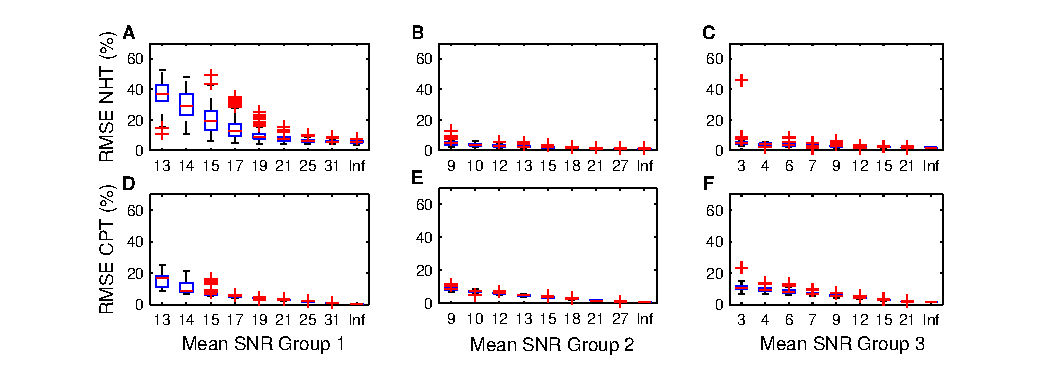
\includegraphics[scale=1]{./Figures/SNRcomparisonFigure.eps}
    \caption{Comparison of the CPT IP estimates to the normalized Hilbert transform incorporating the ensemble empirical mode decomposition for test signal 1 with additive noise. Note; the whiskers show std dev. The red line shows the median, the box cover the data range, except for the outliers shown by red crosses.}
\end{figure*}

The results for the IA estimation are shown in Fig.~\ref{fig:RMSEComparisonSig1_IA}. The error is given as a relative measure with respect to the mean of the actual IA for the respective time periods of each group. For the EEMD, the IA was computed prior to the normalization. The results clearly show the IA estimates of the EEMD are inferior to the CPT. This large errors in the IA estimates for the EEMD are due to the amplitude distortions caused by the iterative sifting process.  
\begin{figure*}[!ht]\label{fig:RMSEComparisonSig1_IA}
    \centering
        \includegraphics[scale=1]{./Figures/IA_RMSE_Sig1.eps}
    \caption{Comparison of the CPT IA estimates to the normalized Hilbert transform for noisy signals.}
\end{figure*}
Figure~\ref{fig:IMFNoNHT} shows a histogram of the IMF indexes for each realization of the test signal for the EEMD. The fifth IMF of the EEMD represented the signal for all of the realizations of the first seven noise levels. For the two highest noise levels, there was also some realizations where the sixth IMF was selected. This is due to intra-mode mixing and explains the outliers in the results for the EEMD.   
\begin{figure}[!ht]\label{fig:IMFNoNHT}
    \centering
        \includegraphics[scale=1]{./Figures/IMFNoFigSig1.eps}
    \caption{IMF index corresponding to the signal.}
\end{figure}


% Focusing on the results from the CPT for the first time group, the variance of the IP estimate begins to increase at a SNR of approximately $14$~dB. These errors occur because the minimum arc length is too short given the noise level. When the minimum arc length is too short, the principal axis of the segment is in the direction of the additive noise rather than following the trajectory of the signal. This can be overcome by using a larger arc length and estimating the tangent vector using more samples. However, increasing the minimum segment size would impact negatively on the higher frequency part of the chirp. For the second time group, as noise is increased, errors increase in a systematic way with an approximate inverse linear relationship to the SNR. For this group, the minimum segment size is sufficient to estimate a satisfactory tangent. Errors in the third group, starting from approximate $7$~dB, are because the SNR is too high for the algorithm to work, regardless of the segment size. Together, these results demonstrate that for relatively simple signals the CPT can estimate IP in the presence of mild disturbances. \todo{DG: we need to consider increasing this discussion of the figure.}
\section{The CPT for Empirical Mode Decomposition}\label{sect:CPTEMDSection}
For low noise signals, the CPT can be used as an alternative to the sifting process of the EMD. The CPT EMD models the signal as
\begin{align}
    y(n) &= x_{0,K}(n) + \sum_{k=1}^{K}x_k(n) + \varepsilon(n) \\
    x_k\left(n\right) &= r_k\left(n\right)cos\left(\phi_k\left(n\right)\right),
\end{align}
where the subscript $k$ indexes the $K$ intrinsic mode functions (IMFs) denoted by $x_k(n)$. The IP, $\phi_k(n)$, for each IMF is estimated using the CPT. In the same manner as the EMD, the IMFs are ordered such that the highest frequency component corresponds to $k=1$. For the first IMF, $x_1(n)$, we can consider $x_{0,1}(n)$ as a modulation term. If $x_{0,1}(n)$ also has modulations, then it can be decomposed into an oscillatory term $x_2(n)$ and an offset (another modulating term) $x_{0,2}(n)$. The process can be repeated until all $K$ oscillatory modes are extracted from $y(n)$, leaving the final offset term or residual $x_{0,K}(n)$.

As we have demonstrated, the IP and IA can be estimated using the CPT without the requirement of sifting. However, the decomposition also relies on an accurate estimate of the offset, $x_{0,k}(n)$. The estimates of the offset from the circle fitting are generally not good enough to perform the decomposition. This is because there may be small drifts in the estimates. To overcome this problem, the CPT EMD uses an empirical method for estimating the offset, in a similar fashion to the standard EMD. It should be noted that the monotonic structure of the IP generally enables an good estimate of $\phi(n)$. Now, assuming the estimate of the IP is accurate, the offset can be found empirically. To show this we first define the signal
\begin{equation}
	\gamma_k(n)=\cos(\phi_k(n)).
\end{equation}   
The extrema of the oscillatory mode $x_k(n)$ occur at the same times as the extrema of $\gamma_k(n)$. Therefore, the estimation of times where extrema occur only relies on an accurate estimate of $\phi_k(n)$. Now consider a noise free signal $y(n)$. The empirical offset can be estimated by 
\begin{equation}
    x_{0,k}(n) = \frac{s_{max,k}(n) + s_{min,k}(n)}{2},
\end{equation}
where $s_{max,k}(n)$ is a cubic spline interpolation through points from $y(n)$ (if $k=1$) or $x_{0,k-1}(n)$ (if $k>1$) corresponding to maxima of $\gamma_k(n)$ and $s_{min,k}(n)$ is another cubic spline interpolation through points of $y(n)$ (if $k=1$) or $x_{0,k-1}(n)$ (if $k>1$) corresponding to minima of $\gamma_k(n)$. The steps of the CPT EMD algorithm are presented in Algorithm~\ref{CPTEMDAlgorithm} and a graphical explanation can be seen in Fig.~\ref{CPT_EMD}.

An advantage of the CPT EMD over the HHT is that the IA structure is maintained and the IP estimate is not subject to the nonlocal effects of the interpolation in the sifting process. In addition, as demonstrated in Section~\ref{sect:NoisySignalsSection} the CPT can estimate the IP in the presence of disturbances thereby alleviating problems from intra-mode mixing. By combining techniques from the HHT and normalized Hilbert transform, an improved and more meaningful EMD is achieved. This demonstrates the advantage of the CPT EMD method. %An examples of using the CPT with an EEG signal is presented in section~\ref{EEGExampleSection}.
% 
\begin{figure}
\centering
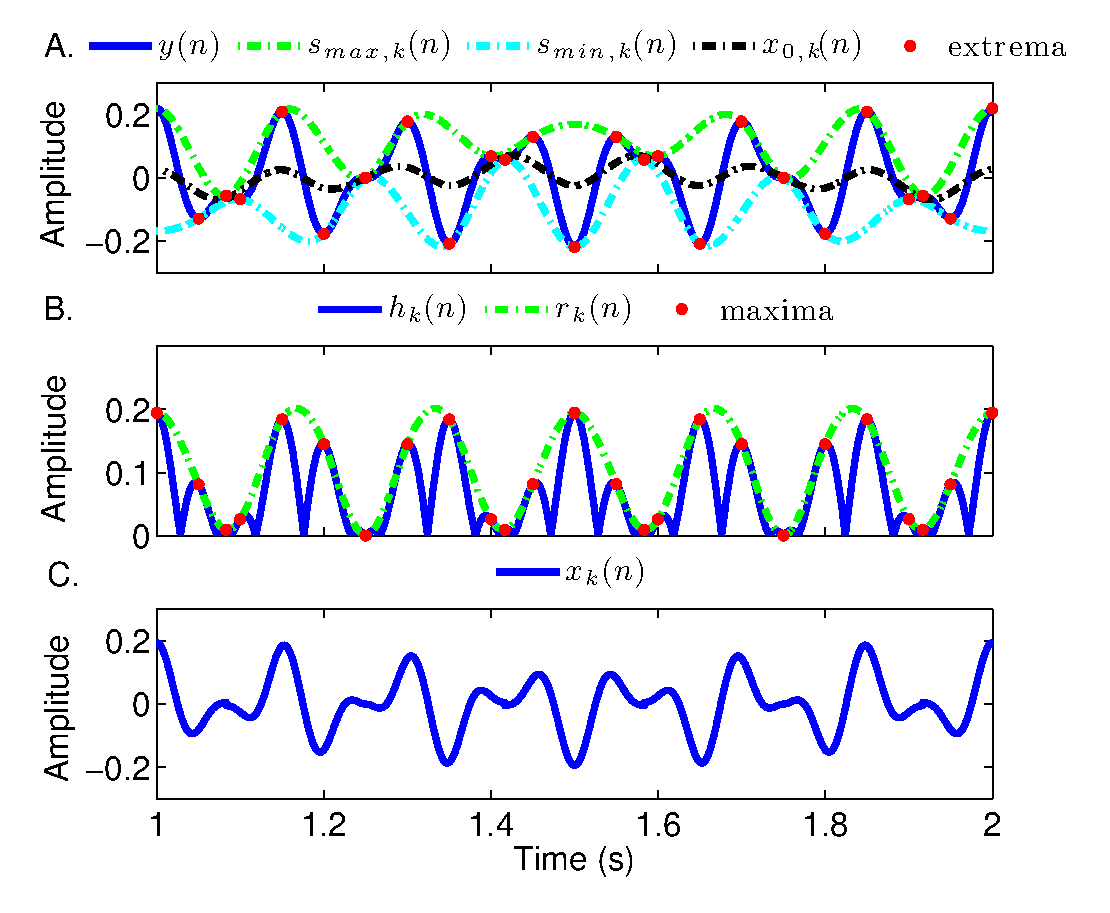
\includegraphics[scale=0.42]{./Figures/CPT_EMD_demo.eps}
\caption[CPT_EMD]{Illustration of the CPT EMD method. The same signal $y(n)$ is used here as was used in Fig.~\ref{fig:HHTDemo}. \textbf{A.} The test signal (blue) with the interpolated maxima and minima lines (green and cyan respectively) and points corresponding the extrema of $cos\left(\phi_1(n)\right)$. \textbf{B.} The absolute value of the test signal demodulated by the empirical offset $x_{0,1}(n)$ (blue), the empirical IA estimate $r_{1}(n)$ (green), and the samples corresponding to extrema of $cos\left(\phi_1\left(n\right)\right)$ (red). \textbf{C.} The first IMF of the CPT EMD decomposition $\tilde{r}_1(n)cos\left(\phi_1\left(n\right)\right)$. Note the empirical offset goes through the points of inflection at $1.25 s$ and $1.75s$, where these points were missed on the first iteration of the sifting process. When comparing the IMF in C. to Fig.~\ref{fig:HHTDemo} D. we can see CPT EMD is superior in preserving the structure of the IA estimate for the decomposition.}
\label{CPT_EMD}
\end{figure}

\begin{algorithm}
\caption{The CPT for EMD}\label{CPTEMDAlgorithm}
\begin{algorithmic}[1]
\State $k=1$
\State use CPT from Algorithm~\ref{CPTAlgorithm} to estimate $\phi_k(n)$ from $y(n)$
\State find local extrema of $cos\left(\phi_k(n)\right)$
\State use extrema to form the splines $s_{min,k}(n)$ and $s_{max,k}(n)$
\State calculate $x_{0,k}(n) = 0.5\left(s_{min,k}(n) + s_{max,k}(n)\right)$
\State find local maxima of $h_k(n)$
\State use maxima to form the spline $r_k(n) = s_{ext,k}(n)$
\While { $x_{0,k}(n)$ is not monotonic }
    \State $k=k+1$
    \State perform CPT on $x_{0,k-1}(n)$ to estimate $\phi_{k}(n)$
    \State repeats steps 3 to 7 to approximate parameters
\EndWhile

\end{algorithmic}
\end{algorithm}

% \begin{figure*}
% \centering
% 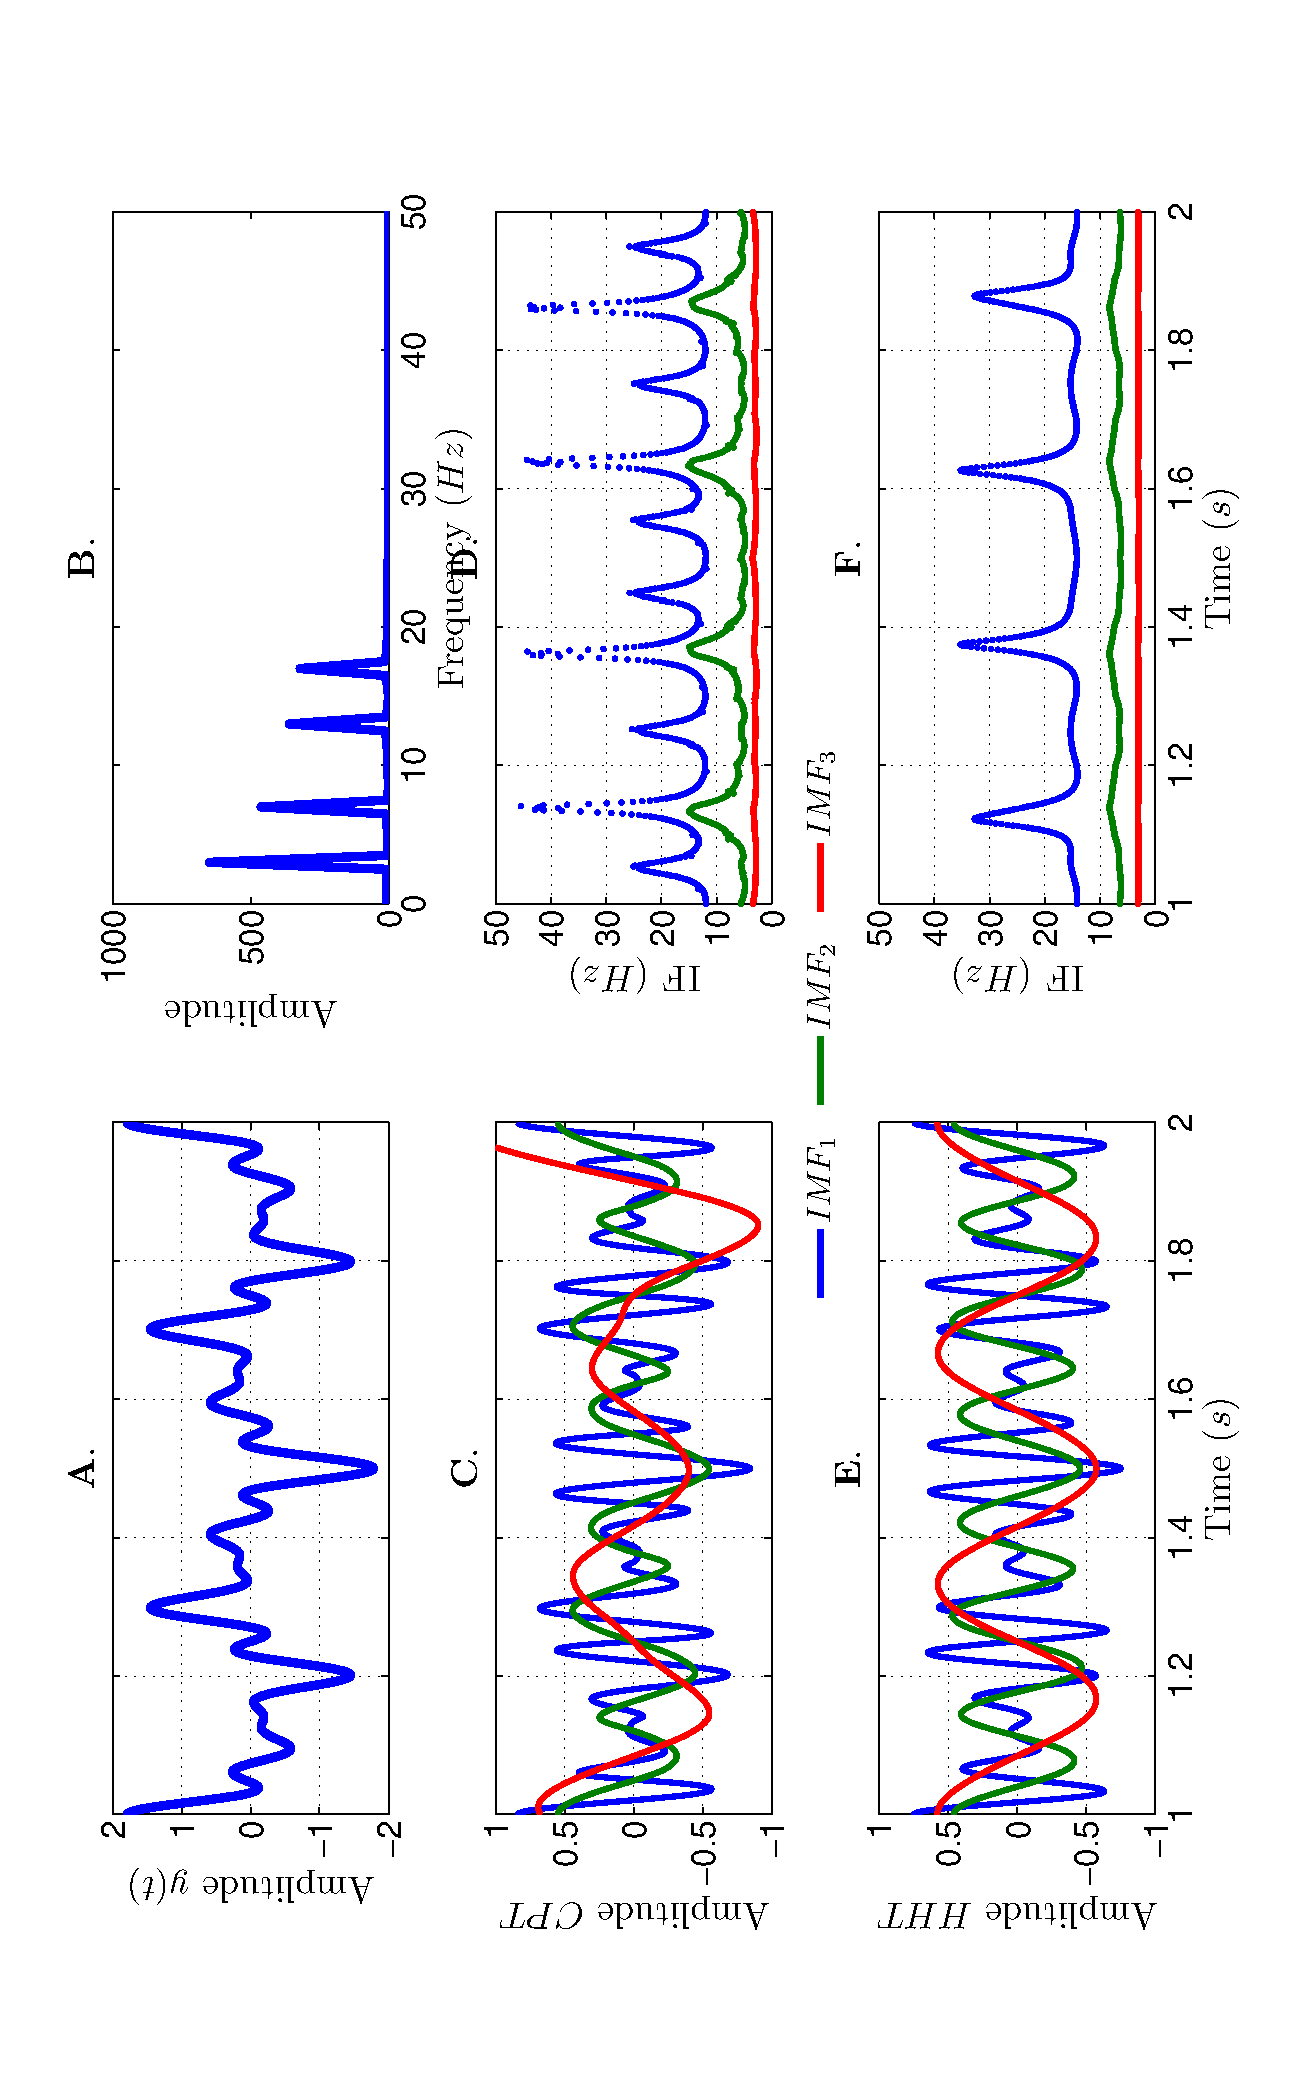
\includegraphics[scale=0.4,angle=-90]{ComparisonCPT2HHT.eps}
% \caption[ComparisonCPT2HHT]{Demonstration of the CPT EMD in comparison to the HHT EMD method. \textbf{A}. The signal $y\left( n \right) = \sum\nolimits_{i = 1}^4 {{a_i}\cos \left( {2\pi {f_i}n} \right)}$ where $f_1 = 3$, $f_2 = 7$, $f_3 = 13$, $f_4 = 17$ Hz and $a_{1,2,3,4} = f_{1,2,3,4}^{-\alpha}$ where $\alpha = 0.4$. \textbf{B}. The spectral components of $y(n)$. \textbf{C}. and \textbf{E}. The first three IMFs calculated using the CPT EMD and HHT EMD methods, respectively. Qualitatively both methods generate similar times series. \textbf{D}. and \textbf{F}. The IFs of the first three IMFs for the CPT EMD and HHT EMD respectively. A clear difference can be seen where the CPT captures more detail with the IF estimates.}
% \label{ComparisonCPT2HHT}
% \end{figure*}



% \section{Examples}
% \subsection{Speech Signal}
% Here we demonstrate how the CPT can be used to analyze speech. We will proceed with a simple example of a person singing `da, da, da, da, da, da, da', increasing in pitch with each `da'. This example was chosen since it is used as an example for demonstrating the HHT, from software publicly available on the Mathworks, Matlab Central File Exchange website~\cite{Tan2008}. This signal provides a good example, as the signal is highly complex, non-stationary, and has different time-frequency scales to study. Fig.~\ref{VoiceDecomp} shows the original signal (9A.) (with no filtering) and the first three IMFs (9C.) of the CPT EMD. The first IMF captures the high frequency details of the signal. As seen in Fig.~\ref{VoiceIMFComparison}, the second IMF captures the fundamental frequency ($F_0$) of the glottal pulses, where the IF steadily increases from approximately 100 Hz in the first `da', to approximately 200 Hz in the final `da'. The third IMF captures the waiver in the $F_0$. This is not the case when using the HHT where inter mode mixing causes problems.
% 
% \begin{figure*}
% \centering
% 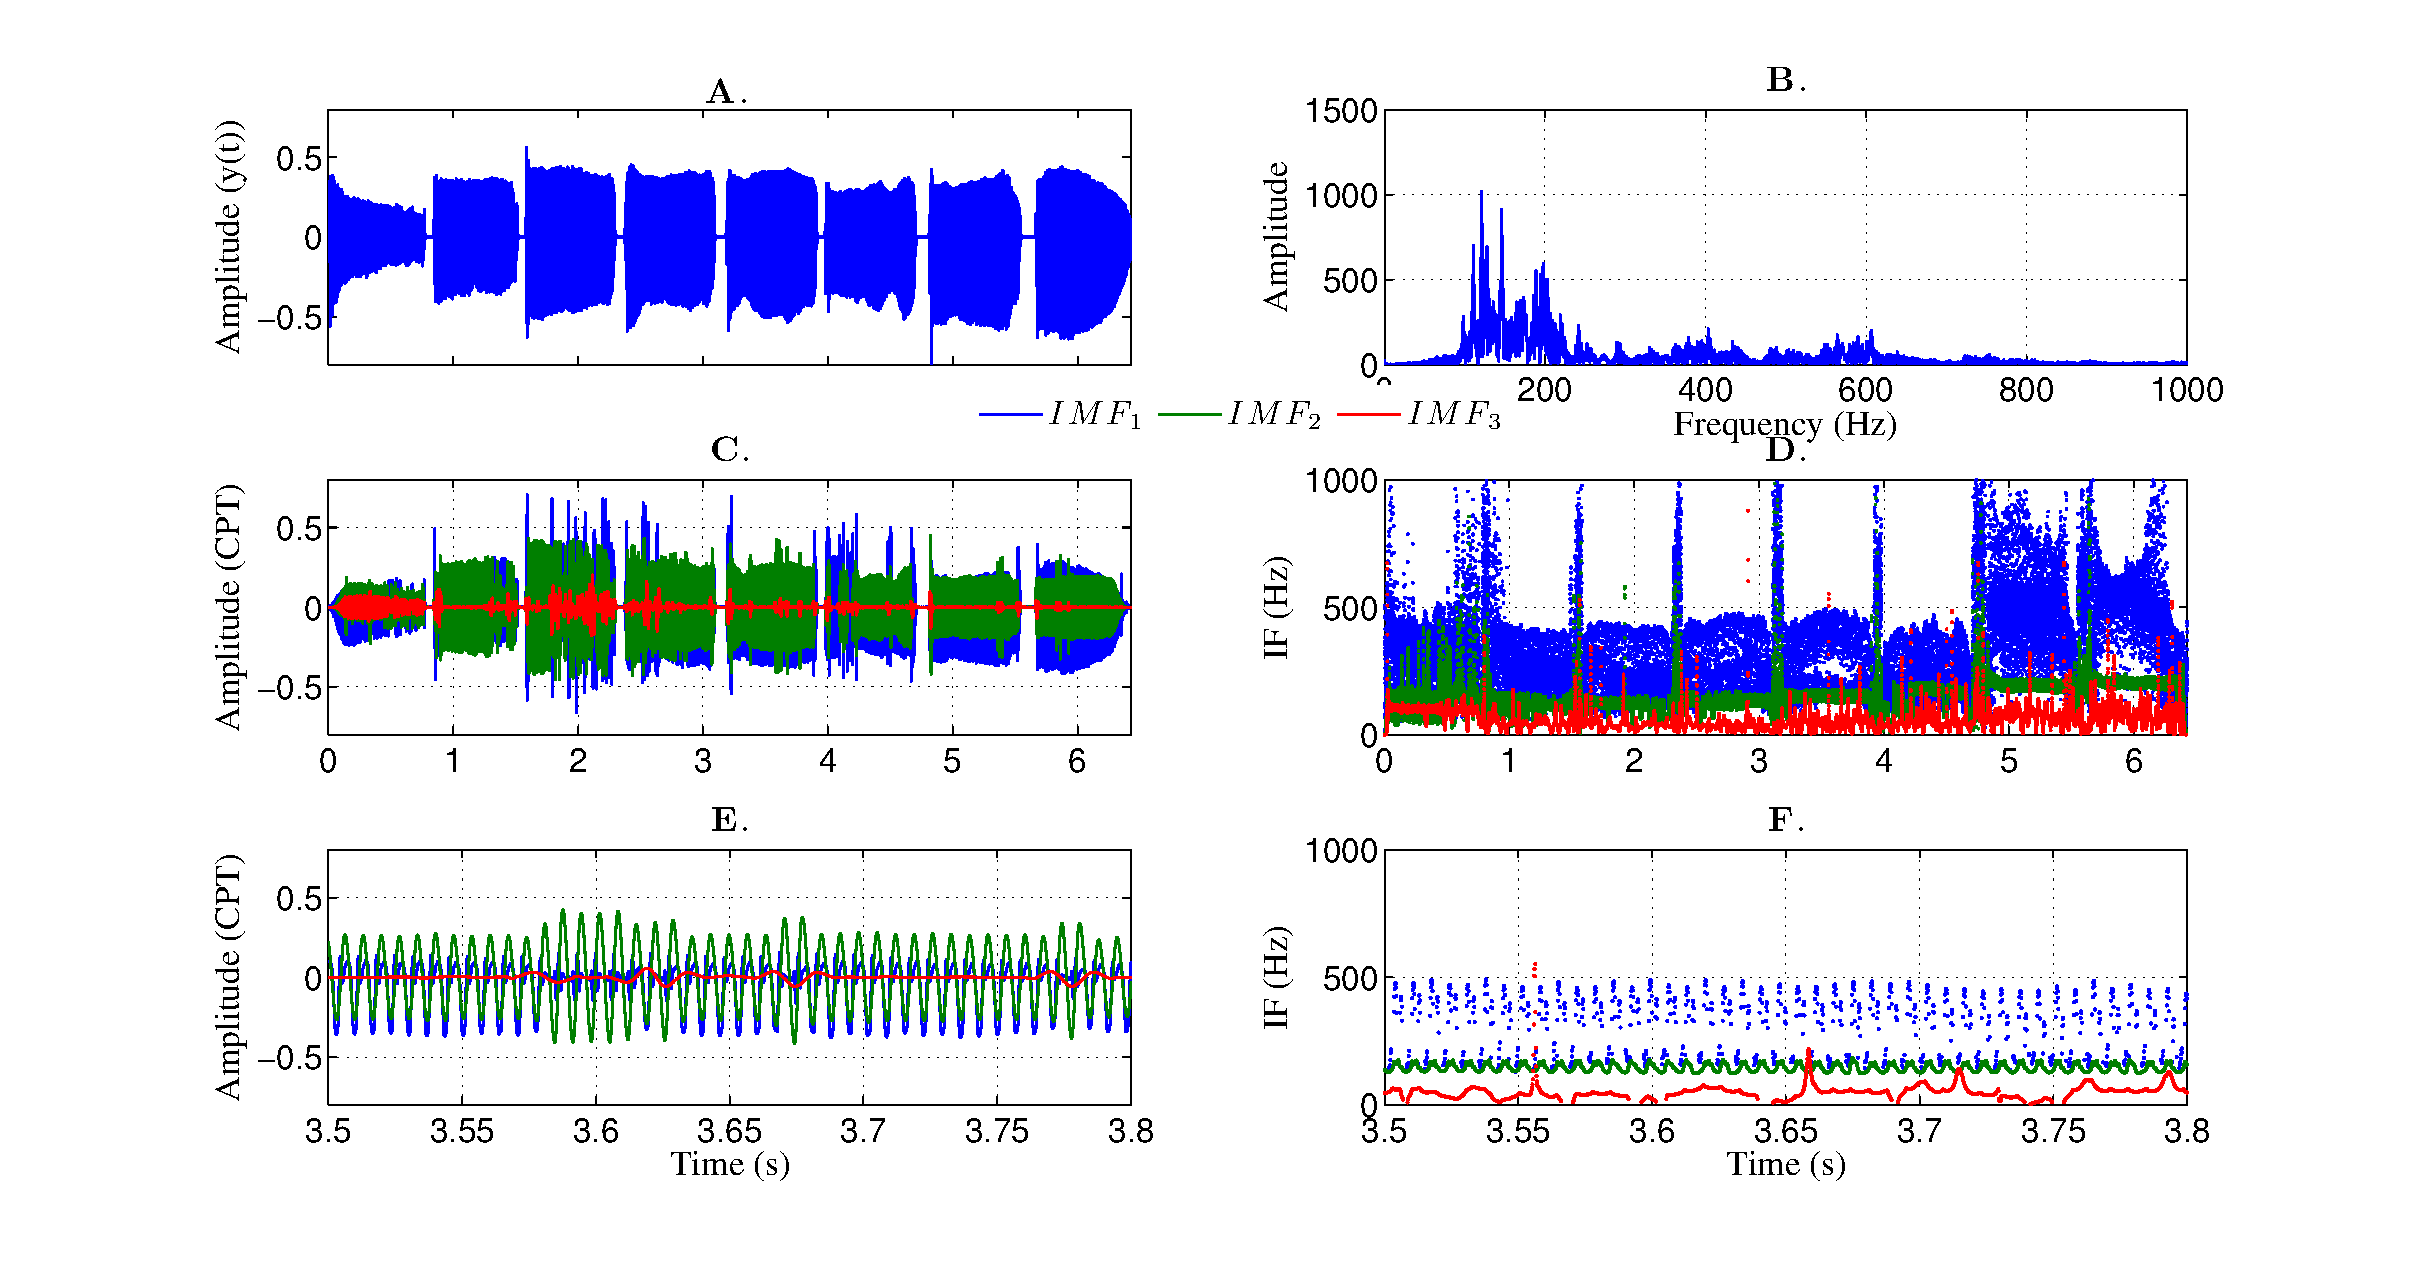
\includegraphics[scale=0.4]{VoiceSignal.eps}
% \caption[VoiceDecomp]{(Figure needs improvement.) Illustration of the CPT EMD on a speech signal. \textbf{A.} The original times series. The signal is recorded in a person singing `da, da, da, da, da', with the tone increasing with each `da'. \textbf{B.} The FFT of the times series. \textbf{C.} and \textbf{E.} The time series of the first three IMFs calculated using the CPT EMD. \textbf{E.} A detailed plot over a finer region of \textbf{C.}. The the first IMF captures the high frequency details of the speech signal, the second IMF captures the fundamental frequency of speech and the third IMF captures variation in the fundamental frequency. \textbf{D.} and \textbf{F.} The IF estimates of the three IMFs. \textbf{F.} shows the details over a smaller time period for the IF estimates.}
% \label{VoiceDecomp}
% \end{figure*}
% 
% \begin{figure*}
% \centering
% 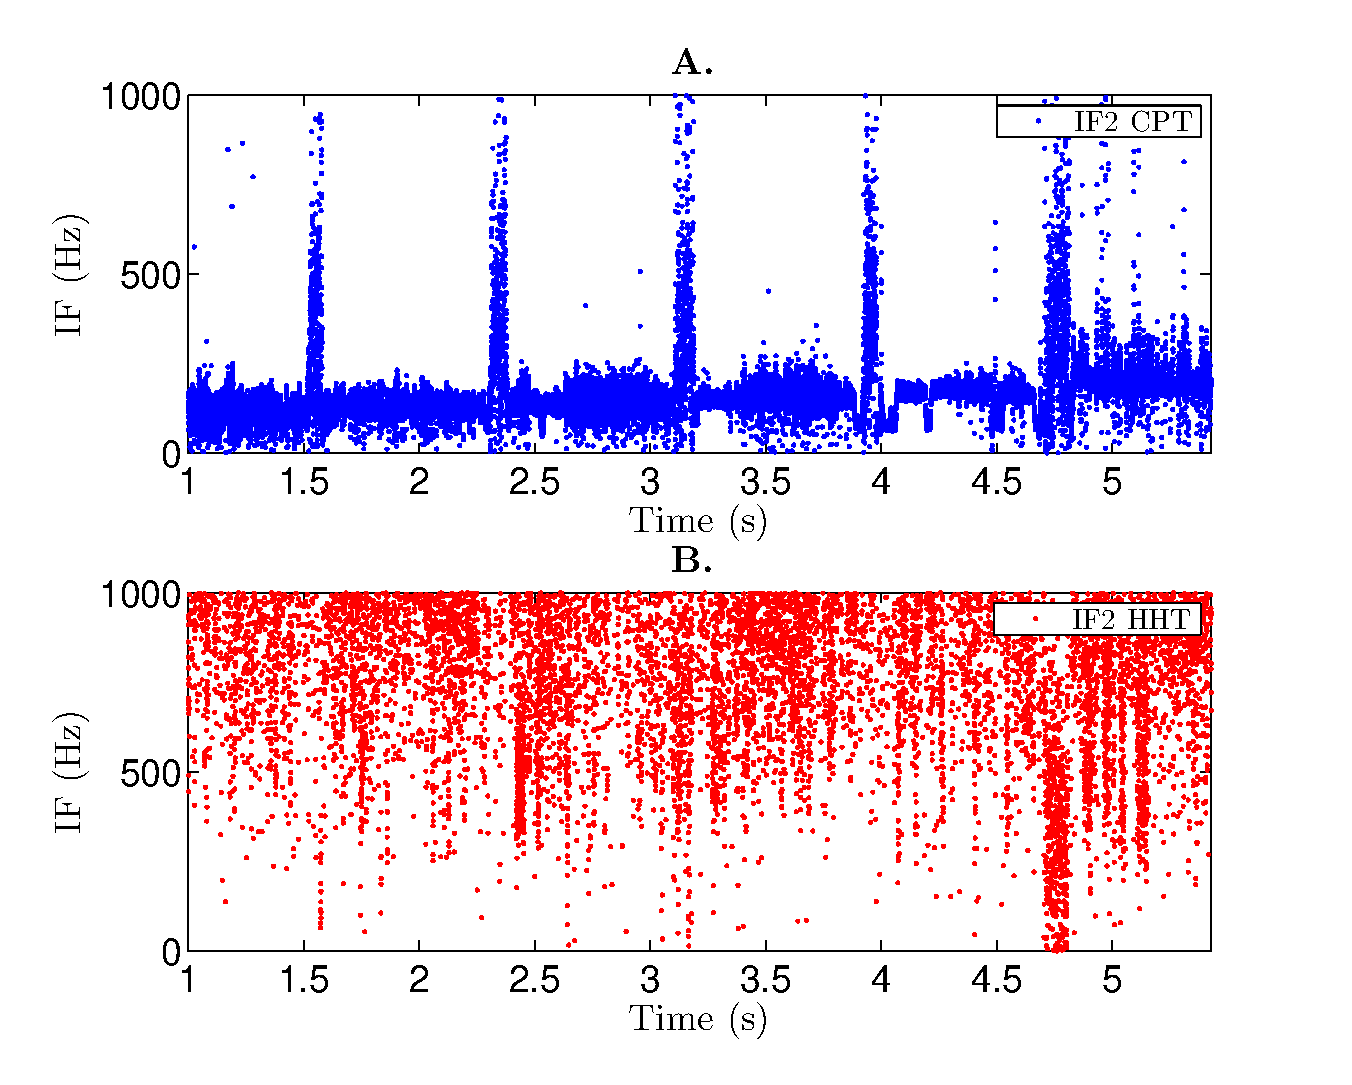
\includegraphics[scale=0.45]{VoiceIMF2Comparison.eps}
% \caption[VoiceIMFComparison]{(Not sure if comparison is fair, as the components may not be equivalent) Comparison of the IF estimates between the HHT EMD and CPT EMD. We compare the second IMF since it represents the fundamental frequency of speech. \textbf{A.} The estimate of the second IMF using the CPT EMD. This shows a clear increase in frequency as the tone of the 'da' increases. \textbf{B.} The second IMF calculated using the HHT EMD. Here we see that the method is not able to capture the detail that was acquired using the CPT.}
% \label{VoiceIMFComparison}
% \end{figure*}
% 
% Cochlear implant speech processing is possible application of this technique. The current model from the leading manufacturer of cochlear implants, Cochlear Ltd., has 22 electrodes implanted in the inner ear. Each electrode is positioned in an area of the cochlea that is sensitive to a different frequency range. For practical reasons only one electrode pair can receive stimulation current at any one time. The choice of the electrode to stimulate is made using speech processing strategies based on Fourier analysis using a filter bank~\cite{Loizou1998}. The CPT EMD offers an alternative where the choice of electrode can be based on the IF estimate and the stimulus activation current based on the IA estimate. The CPT is appropriate for many other signals similar to speech that have periodic aspects with intrawave modulation, that are not well represented by a Fourier basis, and are nonstationary.


% \section{Phase Plane Cusps}\label{sect:PhasePlaneCuspsSection}
% Perhaps the most challenging aspect of estimating instantaneous properties of signals is dealing with points of inflection in the time series, or equivalently for the CPT, cusps in the phase-plane. The difficulty in dealing with cusps lies in whether to interpret them as full oscillations or phase distortions. To illustrate this point, we define three possible scenarios where cusps occur. The first scenario is due additive noise, the second is due to under sampling of the data, the third occurs when cusps are an intrinsic property of signals. The first scenario is a trivial case and cusps introduced by noise should not be be modeled as full oscillations. To deal with this scenario $Q_{min}$ must be sufficiently large to overcome the noise. Examples of how noise effects the performance of the CPT are shown in Section~\ref{sect:NoisySignalsSection}. In practice, the second case is difficult to distinguish from the third case. Nevertheless, appropriate sampling and filtering as a preprocessing step and choosing an appropriate $Q_{min}$ can alleviate problems in with this scenario. Establishing a consistent procedure for dealing with the third scenario is more challenging. To study this we shall show how a simple mixture of two sinusoids can have intrinsic phase-plane cusps. This example is used to show how the CPT can deal with this case and demonstrate how cusps can be modeled as an oscillation or be treated as a phase distortion. The test signal and its Hilbert transform are defined as
% \begin{equation}\label{SamplingSigDef}
%     y\left( t \right) = {a_1}\cos \left( {{\omega _1}t} \right) + {a_2}\cos \left( {{\omega _2}t} \right).
% \end{equation}   
% To study where cusps occur, we first examine loops in the phase-plane that do not enclose the origin. As the signal goes through such a loop, the Hilbert phase slows, stops, reverses, stops again, and then proceeds forward. For the test signal, the time interval where the phase is decreasing (reversing) can be solved analytically by finding the period between stationary points of the Hilbert phase. The stationary points can be found by solving for times where the derivative of the IP is zero. For the test signal, an analytic form of the Hilbert phase can be found. The derivative of the analytic Hilbert phase is 
% \begin{eqnarray}
%     \frac{d\phi_y(t)}{dt}&=&0.5(\omega_2 + \omega_1) + 0.5(\omega_2 - \omega_1)\frac{a_2^2-a_1^2}{A^2(t)} \\
%     A^2(t) &=& a_1^2 + a_2^2 + 2a_1^2a_2^2cos((\omega_2-\omega_1)t).
% \end{eqnarray}
% The derivative of the Hilbert phase is zero where
% \begin{equation}\label{StationaryPhaseTimes}
%     t=\frac{1}{\omega_2-\omega_1}\arccos\left(-\frac{a_1^2\omega_1 + a_2^2\omega_2}{(\omega_2 +
%     \omega_1)a_1^2a_2^2}\right)+\frac{1}{\omega_2-\omega_1}2\pi k,
% \end{equation}
% where $k=1,2,...$ and the phase reversal period is (see Appendix~\ref{ReversalPeriodDerivation} for derivation) 
% \begin{eqnarray}\label{PhaseReversalPeriod}
%     T=\frac{2}{\omega_2-\omega_1}\arccos\left(g\left(a_1,a_2,\omega_1,\omega_2\right)\right) \\ 
% g\left(a_1,a_2,\omega_1,\omega_2\right) = \frac{a_1^2\omega_1 + a_2^2\omega_2}{(\omega_2 +
%     \omega_1)a_1^2a_2^2}.
% \end{eqnarray}
% For this test signal the sampling rate, $F_s$, must satisfy
% \begin{equation}
%     F_s \ge \frac{2}{T}
% \end{equation}
% to guarantee no cusps will be present. If $g>1$, then it becomes a complex quantity and cusps will be present irrespective of the sampling frequency. These are intrinsic cusps of the signal. If $g=1$ the cusps will be pointed and the CPT will map them as full oscillations. Small errors will occur when the segment used to fit the circle overlaps the point of the cusp. These errors occur because the fitted circle center will be on the incorrect side of the arc at the cusp. These errors will be detected and corrected by the methods explained in Section~\ref{sect:ComputingCPTSection}. However, when $g \gg 1$ the cusps become rounded and the CPT no longer maps them as full oscillations. 
% 
% Examples of the CPT mapping for $g<1$, $g=1$ and $g>1$ are shown in Fig.~\ref{Cusps}. The left column of the Figure shows $y(n)$ (plotted with dashed black line) and $x_1(n)$ (in red). The IP estimates in this column where found using $Q=4$. The CPT mapped the small loops (upper plot in column) and the pointed cusps (middle plot) as full oscillations. When the cusp become rounded in the lower plot the CPT was unable to map it as a full oscillation. 
% 
% The middle columns shows $y(n)$ plotted with $x_1(n)$, but this time $Q$ was fixed at $110$. The larger segment size has an effect of high pass filtering the phase-plane representation of the data. The upper plot of the column shows that the small loops were not captured by with the larger arc size. However, the lower plot of the column shows the larger arc was able find good fits when the cusps become rounded.
% The transition between where cusps are pointed and where they are rounded seems like a good delineator between where they should be modeled by full oscillations and phase distortions. Further work is required to improve mappings to account for transitions from pointed to rounded cusps. 
% \begin{figure*}
%     \centering
%         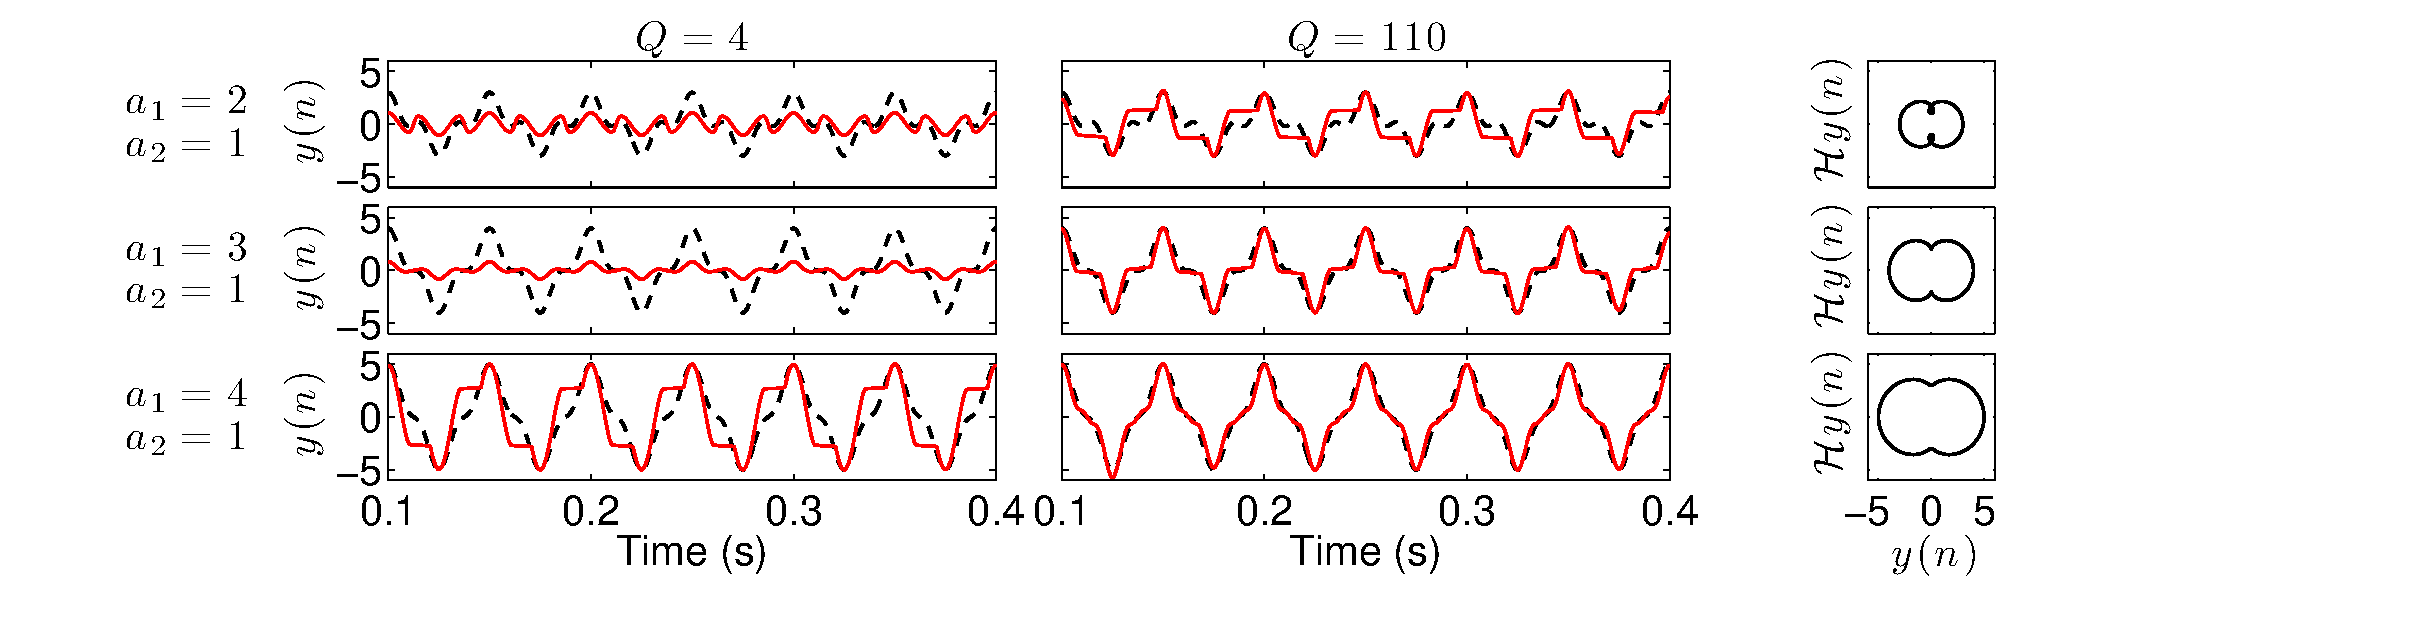
\includegraphics[scale=0.4]{DemonstrateCusps.eps}
%             \caption[Cusps]{Examples of phase-plane cusps}
%         \label{Cusps}
% \end{figure*}
% The examples in Fig.~\ref{Cusps} show that dealing with cusps is challenging. It is important to deal with cusp in a consistent manner, regardless of the method estimating instantaneous properties of signals. Although errors may occur at data segments with rounded cusps, the CPT is consistent in the way it deals with this problem. If possible, data should be high pass filtered, cutting any unwanted low frequency high amplitude components to avoid this problem. This has an effect of contracting these phase-plane representation of the signal, increasing the accuracy of the mapping. By setting a low-pass filter to remove unwanted high frequency components of the signal and set the minimum arc length to half the number of samples in the period of the highest frequency component then the CPT will perform well. 
% 
% \section{Neural Oscillations Example}\label{EEGExampleSection}
% Analysis of instantaneous phase (IP) for EEG signals is an important and expanding area of neuroscientific research, where phase synchronisation has been used to study various forms of cognitive neurodynamics~\cite{Varela2001}. Estimating IP of the brain's rhythms is nontrivial since there highly nonstationary, of a nonlinear origin, has many inflection points and amplitude and frequency modulations. Previously, IP estimates from neural oscillations have been restricted to narrow-band signals. Typically, a narrow pass-band filter is used and the IP is estimated using the Hilbert transform of the filtered signal. Alternatively, the complex Morlet wavelet is commonly used to extract the analytic signal~\cite{LeVanQuyen2001}. Narrow-band filtering has serious consequences that are often overlooked in EEG signal processing. When using narrow-band filtering, one must assume the signal has a sinusoidal basis (or other basis for wavelets). This is obviously not true for signals generated in the brain. Additional problems arise when artifacts or sharp edges occur in signals. The filtered time series will exhibit a ringing from the impulse response of the filter, which will lead to erroneous phase estimates. 
% 
% Fig.~\ref{fig:EEGExample} shows an example of the CPT EMD of an epileptic seizure recorded with intracranial EEG. The data is a referential recording sampled at 4069 Hz from an electrode at the epileptic focus. The data was preprocessed using a median filter ($20^{th}$ order) and low-pass filtered with a cut-off at $45$ Hz. The minimum arc length $Q_{min}$ was set to $15$ and the maximum arc length $Q_{max}$ was $150$. The arc length was incremented in steps of $4$ samples. The IFs of the decomposed signal show a highly detailed frequency structure.
% 
% The brain's rhythms have specific oscillatory bands that are associated with various cognitive states. For example, phase synchronization of the gamma rhythm (40-90 Hz) between sensory cortices has been implicated as a mechanism for binding of incoming multi-sensory information into a single percept (ref). Also, phase resetting of the alpha rhythm (8-12 Hz) has been implicated in processing sensory information. On a finer scale, phase precession of single neuron theta oscillations (3-8 Hz) has been shown to encode information on navigation and place. Since there is known frequency bands associated with these processes data can be filtered and the CPT can be used as method of correcting phase estimates. 
% \begin{figure*}
% \centering
% 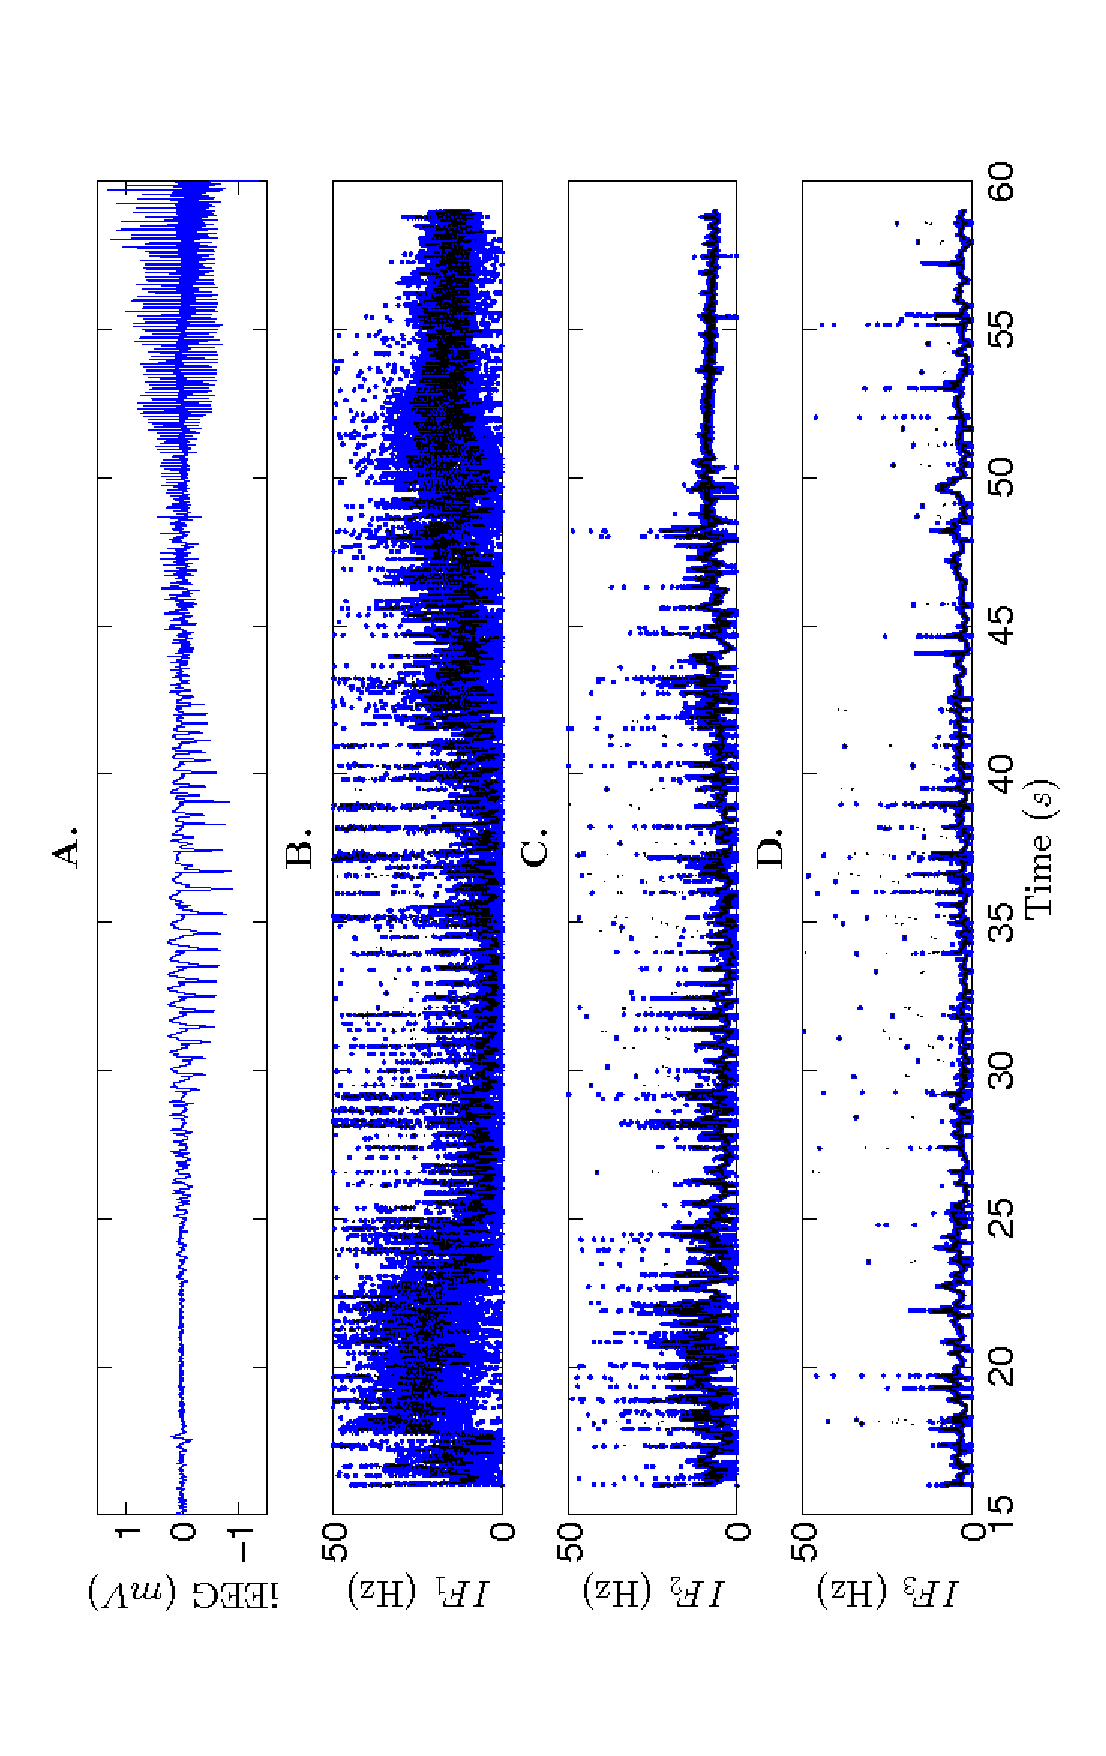
\includegraphics[scale=0.4,angle=-90]{EEGExample.eps}
% \caption[EEGExample]{(Figure also needs some improvement) Illustration of the application of the CPT for EEG analysis. \textbf{A}. The EEG time series at the onset of an epileptic seizure. \textbf{B}, \textbf{C} and \textbf{D} show the IF estimates for the first three IMFs (blue dots) and a trend (black dots) calculated using a median filter of order 30. \textbf{B} Highlights the nonstationarity of the frequency content of the spiking discharges. \textbf{C}. Illustrates how the occurrence of epileptic spikes becomes highly regular at 50~s and how the spiking frequency then slowly reduces. \textbf{D} Illustrates the variation in the spiking frequency.}
% \label{fig:EEGExample}
% \end{figure*}
% 
% \begin{figure*}[htbp]
%     \centering
%         \includegraphics[scale=0.4]{EEG_time_freq_fig.eps}
%     \caption{This is the short time histogram of the IF estimate. IF estimates are windowed and then binned. Window overlap is 75 percent and window size is about 1 second. IMFs are ordered from top to bottom. }
%     \label{fig:timefreqplot}
% \end{figure*}
% 
% \begin{figure}[htbp]
%     \centering
%         \includegraphics[scale=.4]{EEGDecompFig.eps}
%     \caption{This figure shows how data is well represented by the IMFs. Just want to show that cusps are present but we can see data is well represented.}
%     \label{fig:EEGdecomp}
% \end{figure}

\section{Discussion}\label{sect:DiscussionSection}
We have presented a new method for estimation of instantaneous properties of nonstationary signals. The novelty in our method is in the demodulation of the signal in the phase-plane. Demodulating in the phase-plane has advantages over methods in the time domain such as, 
\begin{itemize}
    \item circle fitting is easier then fitting sinusoids (fewer parameters to find),
    \item circle fitting enforces a quadrature structure to data,
    \item errors in circle center and radius do not equate to errors in the phase estimate,
    \item mapping is equivalent to translation of origin so relative distance mismatch can be used,
    \item the use of a model allows for introduction of a disturbance term,
    \item and it provides an intuitive representation.
\end{itemize}
The inclusion of signal model and a disturbance term will allow for benchmarking and quantitative improvements to be made.

A major benefit for the CPT over the HHT is the consistency with how handles inflections in a time series and the ability preserve IA estimates. The consistency in dealing with inflection is due to the more local demodulation and estimation of the signal properties. The preservation of the IA estimate is because the CPT does require the iterative sifting to extract the IMFs. The CPT can be applied to many areas are signal processing and engineering where the HHT has been previously used. At the time of publishing the original HHT algorithm had been cited more than $2600$ times demonstrating it's wide applicability.

Successful implementation of the CPT requires high sampling rates and high SNRs. In addition, in the current implementation of the algorithm errors are unavoidable at phase-plane cusps. These short comings can be addressed through careful data acquisition and appropriate pre-processing. Also, the parameters specifying the arc lengths must be chosen carefully. For noisy signals the minimum arc length is a critical parameter and should set sufficiently large to overcome the noise. We have demonstrated that the CPT can model very complicated signals like the EEG with excellent results. Further work should be directed improving estimates around phase-plane cusps.
Further research in this area should be directed towards find improved circle fitting algorithms, further developing criteria to find circle estimates that best describes the instantaneous properties of signals, and improving estimates around phase-plane cusps.

% \begin{itemize}
%   \item Conditions - most signals will satisfy, interpretation.. measurement
%   \item Mention possible applications.
%   \item Using the CPT as a filter, where we can make random draws around the the point of interest to create a distribution of circle parameters (not sure this random draw will perform at a cusp point).
%   \item We can take our segment so that the current sample starts at the end and translates to the start. This will improve the phase estimates as we approach cusps.  
%   \item Hilbert-Huang transform and its applications By Norden Eh Huang, Samuel S. Shen, has a section on the open problems associated with the hht. I think we address some of them. 
%   \item completeness
% \end{itemize}


\section{Conclusion}\label{sect:ConclusionSection}
We have presented a new method for estimating instantaneous amplitude, phase, and frequency from nonlinear, nonstationary time series. This new approach extends the concepts introduced by Huang et al.~\cite{Huang1998} by providing a more local estimate of the instantaneous phase. We demonstrated how the sifting process can have problems with inflections in signals due to the non-local demodulation. The Circular Phase Transform (CPT) overcomes this problem by estimating more local properties. We have demonstrated how our method can be incorporated into the empirical mode decomposition (EMD) allowing for a meaningful estimates of the instantaneous amplitude of intrinsic mode functions (IMFs). The CPT can be applied to a wide range of signal processing problems, such as nonlinear system identification, speech processing, EEG analysis etc., where the HHT has been used. 


% The results for the second test signal are shown in Figure~\ref{fig:RMSEComparisonSig2}. 
% \begin{figure*}[!ht]\label{fig:RMSEComparisonSig2}
%     \centering
%         \includegraphics[scale=1]{./Figures/SNRcomparisonFigureSig2.eps}
%     \caption{Comparison of the CPT IP estimates to the normalized Hilbert transform for noisy signals. Note; the whiskers show std dev. The red line shows the median, the box cover the data range, except for the outliers shown by red crosses.}
% \end{figure*}


%\section{Instantaneous Amplitude Estimates}
%Perhaps the most significant benefit of using the CPT over the HHT is the ability to extract meaningful IA estimates. To compare the techniques we use a signal that is composed of two sinusoids (from Eq.~\ref{SamplingSigDef} with $f_1 = 7$ Hz, $f_2 = 17$ Hz ($\omega = 2\pi f$) and $a_{1,2} = f_{1,2}^{-1}$ since mixture of sinusoids can be represented as a monocomponent signal with a distorted time varying phase and amplitude.
%\begin{eqnarray}\label{DistortedSinusoids}
%% \nonumber to remove numbering (before each equation)
%  y\left( t \right) &=& {a_1}\cos \left( {{\omega _1}t} \right) + {a_2}\cos \left( {{\omega _2}t} \right) \nonumber \\
%   &=& {a_1}\cos \left( {\left( {\Omega  - \Phi } \right)t} \right) + {a_2}\cos \left( {\left( {\Omega  + \Phi } \right)t} \right) \nonumber \\
%   &=& b\left( t \right)\cos \left( {\Omega t + \Theta \left( t \right)} \right). \nonumber
%\end{eqnarray}
%where
%\begin{eqnarray}
%% \nonumber to remove numbering (before each equation)
%  \Theta \left( t \right) &=& {\arctan}\left( {\frac{{\left( {{a_1} - {a_2}} \right)\tan \left( {\Phi t} \right)}}{{{a_1} + {a_2}}}} \right) \hfill \\
%  b\left( t \right) &=& \sqrt {{a_1}^2 + {a_2}^2 + 2{a_1}{a_2}\cos \left( {2\Phi t} \right)}  \hfill
%\end{eqnarray}
%The term $b(t)$ is a scaled version of the true IA. The scaling is due to the offset being absorbed into the cosine term in eq~\ref{DistortedSinusoids}. Under the assumption that we can estimate the instantaneous phase accurately, we can remove the scaling on $b(t)$ to compare IA estimates by letting
%\begin{equation}\label{RemoveScaling}
%\bar b\left( t \right) = \psi \left( t \right)\left( {b\left( t \right) - \sqrt {{a_1}^2 + {a_2}^2 - 2{a_1}{a_2}} } \right)
%\end{equation}
%\begin{equation}\label{}
%    
%\end{equation}


% An example of a floating figure using the graphicx package.
% Note that \label must occur AFTER (or within) \caption.
% For figures, \caption should occur after the \includegraphics.
% Note that IEEEtran v1.7 and later has special internal code that
% is designed to preserve the operation of \label within \caption
% even when the captionsoff option is in effect. However, because
% of issues like this, it may be the safest practice to put all your
% \label just after \caption rather than within \caption{}.
%
% Reminder: the "draftcls" or "draftclsnofoot", not "draft", class
% option should be used if it is desired that the figures are to be
% displayed while in draft mode.
%
%\begin{figure}[!t]
%\centering
%\includegraphics[width=2.5in]{myfigure}
% where an .eps filename suffix will be assumed under latex,
% and a .pdf suffix will be assumed for pdflatex; or what has been declared
% via \DeclareGraphicsExtensions.
%\caption{Simulation Results}
%\label{fig_sim}
%\end{figure}

% Note that IEEE typically puts floats only at the top, even when this
% results in a large percentage of a column being occupied by floats.
%
% An example of a double column floating figure using two subfigures.
% (The subfig.sty package must be loaded for this to work.)
% The subfigure \label commands are set within each subfloat command, the
% \label for the overall figure must come after \caption.
% \hfil must be used as a separator to get equal spacing.
% The subfigure.sty package works much the same way, except \subfigure is
% used instead of \subfloat.
%
%\begin{figure*}[!t]
%\centerline{\subfloat[Case I]\includegraphics[width=2.5in]{subfigcase1}%
%\label{fig_first_case}}
%\hfil
%\subfloat[Case II]{\includegraphics[width=2.5in]{subfigcase2}%
%\label{fig_second_case}}}
%\caption{Simulation results}
%\label{fig_sim}
%\end{figure*}
%
% Note that often IEEE papers with subfigures do not employ subfigure
% captions (using the optional argument to \subfloat), but instead will
% reference/describe all of them (a), (b), etc., within the main caption.

% An example of a floating table. Note that, for IEEE style tables, the
% \caption command should come BEFORE the table. Table text will default to
% \footnotesize as IEEE normally uses this smaller font for tables.
% The \label must come after \caption as always.
%
%\begin{table}[!t]
%% increase table row spacing, adjust to taste
%\renewcommand{\arraystretch}{1.3}
% if using array.sty, it might be a good idea to tweak the value of
% \extrarowheight as needed to properly center the text within the cells
%\caption{An Example of a Table}
%\label{table_example}
%\centering
%% Some packages, such as MDW tools, offer better commands for making tables
%% than the plain LaTeX2e tabular which is used here.
%\begin{tabular}{|c||c|}
%\hline
%One & Two\\
%\hline
%Three & Four\\
%\hline
%\end{tabular}
%\end{table}

% Note that IEEE does not put floats in the very first column - or typically
% anywhere on the first page for that matter. Also, in-text middle ("here")
% positioning is not used. Most IEEE journals use top floats exclusively.
% Note that, LaTeX2e, unlike IEEE journals, places footnotes above bottom
% floats. This can be corrected via the \fnbelowfloat command of the
% stfloats package.


\appendices
% \section{Phase Reversal Period Derivation}\label{ReversalPeriodDerivation}
% From Eq.~\ref{StationaryPhaseTimes} to stationary phase times are
% \begin{equation}
%     t=\frac{1}{\omega_2-\omega_1}\arccos\left(-\frac{a_1^2\omega_1 + a_2^2\omega_2}{(\omega_2 +
%     \omega_1)a_1^2a_2^2}\right)+\frac{1}{\omega_2-\omega_1}2\pi k.
% \end{equation}
% Due to the $2\pi$ periodic nature of $\arccos$ we can also write
% \begin{eqnarray}
%     t= \left(2\pi - \frac{1}{\omega_2-\omega_1}\arccos\left(-\frac{a_1^2\omega_1 + a_2^2\omega_2}{(\omega_2 +
%     \omega_1)a_1^2a_2^2}\right)\right) \\ \nonumber
% +\frac{1}{\omega_2-\omega_1}2\pi k.
% \end{eqnarray}
% The time between the first and second phase reversal is given by
% \begin{equation}\label{T}
%     T = t_1 - t_2,
% \end{equation}
% where
% \begin{eqnarray}
%     t_1 &=& 2\pi - \frac{1}{\omega_2-\omega_1}\arccos\left(-\frac{a_1^2\omega_1 + a_2^2\omega_2}{(\omega_2 +
%         \omega_1)a_1^2a_2^2}\right)  \label{t_1} \\
%     t_2 &=& \frac{1}{\omega_2-\omega_1}\arccos\left(-\frac{a_1^2\omega_1 + a_2^2\omega_2}{(\omega_2 +
%         \omega_1)a_1^2a_2^2}\right). \label{t_2}
% \end{eqnarray}
% By substituting Eqs.~\ref{t_1} and Eqs.~\ref{t_2} into Eq.~\ref{T} and making simplifications we get Eq.~\ref{PhaseReversalPeriod} as required. 



% (2\pi - \frac {1}{\omega_2-\omega_1}\arccos\left(-\frac{a_1^2\omega_1 + a_2^2\omega_2}{(\omega_2 +
%       \omega_1)a_1^2a_2^2}\right))- \frac{1}{\omega_2-\omega_1}\arccos\left(-\frac{a_1^2\omega_1 + a_2^2\omega_2}{(\omega_2 +
%       \omega_1)a_1^2a_2^2}\right) \\
%       &=& \frac{2}{\omega_2-\omega_1}\left(\pi - \arccos\left(-\frac{a_1^2\omega_1 + a_2^2\omega_2}{(\omega_2 +
%       \omega_1)a_1^2a_2^2}\right) \right) \\
%       &=& \frac{2}{\omega_2-\omega_1}\arccos\left(\frac{a_1^2\omega_1 + a_2^2\omega_2}{(\omega_2 +
%       \omega_1)a_1^2a_2^2}\right)
%   \end{eqnarray}

% use section* for acknowledgement
\section*{Acknowledgment}
This research was funded by the Australian Research Council (Linkage Project LP0560684). The Bionic Ear Institute acknowledges the support it recieves from the Victorian State Government through the Operational Infrastructure Support Program. Dean Freestone would like to thank the University of Melbourne's Scholarships Office for the Postgraduate Overseas Research Experience Scholarship and the Harold Mitchell Foundation for a traveling scholarship for supporting this research. In addition, Dean Freestone would like to thank Dr. Mark van Rossum for hosting him whilst visiting the University of Edinburgh where this work was completed. Additional thanks go to Stefan Mauger for many helpful discussions and feedback.

%\ifCLASSOPTIONcaptionsoff
%  \newpage
%\fi



% references section

\bibliographystyle{IEEEtran}
\bibliography{IEEEabrv,CPT}


% biography section
%
% If you have an EPS/PDF photo (graphicx package needed) extra braces are
% needed around the contents of the optional argument to biography to prevent
% the LaTeX parser from getting confused when it sees the complicated
% \includegraphics command within an optional argument. (You could create
% your own custom macro containing the \includegraphics command to make things
% simpler here.)
%\begin{biography}[{\includegraphics[width=1in,height=1.25in,clip,keepaspectratio]{mshell}}]{Michael Shell}
% or if you just want to reserve a space for a photo:

% \begin{IEEEbiography}{Dean R. Freestone}
% Biography text here.
% \end{IEEEbiography}
% 
% % if you will not have a photo at all:
% \begin{IEEEbiography}{David B. Grayden}
% Biography text here.
% \end{IEEEbiography}
% 
% % insert where needed to balance the two columns on the last page with
% % biographies
% %\newpage
% 
% \begin{IEEEbiography}{Anthony N. Burkitt}
% Biography text here.
% \end{IEEEbiography}
% 
% \begin{IEEEbiography}{Alan Lai}
% Biography text here.
% \end{IEEEbiography}
% 
% \begin{IEEEbiography}{Tim Nelson}
% Biography text here.
% \end{IEEEbiography}
% 
% \begin{IEEEbiography}{Levin Kuhlman}
% Biography text here.
% \end{IEEEbiography}

% that's all folks
\end{document} 